% ═══════════════════════════════════════════════════════════════
%  Weekly Meeting — 10 April 2026
%  Tissue-Interface Beamlet Analysis for ADoTA
%  Author: Mikołaj Stryja
% ═══════════════════════════════════════════════════════════════
\documentclass[aspectratio=169, 10pt]{beamer}

% ── Theme & colours ─────────────────────────────────────────
\usetheme{Madrid}
\usecolortheme{default}
\definecolor{tudelft}{RGB}{0,100,172}
\setbeamercolor{structure}{fg=tudelft}
\setbeamercolor{title}{fg=white,bg=tudelft}
\setbeamercolor{frametitle}{fg=white,bg=tudelft}
\setbeamertemplate{navigation symbols}{}
\setbeamertemplate{footline}{%
  \leavevmode\hbox{%
    \begin{beamercolorbox}[wd=.33\paperwidth,ht=2.5ex,dp=1ex,center]{author in head/foot}%
      \usebeamerfont{author in head/foot}\insertshortauthor
    \end{beamercolorbox}%
    \begin{beamercolorbox}[wd=.34\paperwidth,ht=2.5ex,dp=1ex,center]{title in head/foot}%
      \usebeamerfont{title in head/foot}\insertshorttitle
    \end{beamercolorbox}%
    \begin{beamercolorbox}[wd=.33\paperwidth,ht=2.5ex,dp=1ex,right]{date in head/foot}%
      \usebeamerfont{date in head/foot}\insertframenumber{}/\inserttotalframenumber\hspace*{2ex}
    \end{beamercolorbox}}%
  \vskip0pt%
}

% ── Packages ────────────────────────────────────────────────
\usepackage{graphicx}
\usepackage{booktabs}
\usepackage{amsmath,amssymb}
\usepackage{siunitx}
\usepackage{tikz}
\usetikzlibrary{arrows.meta,positioning,calc}
\usepackage{xcolor}
\usepackage{multirow}
\graphicspath{{figures/}}

% ── Meta ────────────────────────────────────────────────────
\title[ADoTA Tissue-Interface Analysis]{Tissue-Interface Beamlet Analysis\\[4pt]
{\small Effect of Bragg-Peak Neighbourhood Heterogeneity\\on ADoTA Dose-Prediction Accuracy}}
\author[M.~Stryja]{Mikołaj Stryja}
\institute{Department of Radiation Science \& Technology}
\date{10 April 2026}

% ════════════════════════════════════════════════════════════
\begin{document}

% ── Title ───────────────────────────────────────────────────
\begin{frame}[plain]
  \titlepage
\end{frame}

% ── Outline ─────────────────────────────────────────────────
\begin{frame}{Outline}
  \tableofcontents
\end{frame}

% ════════════════════════════════════════════════════════════
\section{Motivation}
% ════════════════════════════════════════════════════════════

\begin{frame}{Motivation}
  \begin{itemize}
    \item ADoTA (DoTA3D\_v3) predicts single-beamlet proton dose distributions
          from CT\,+\,beam flux input using a 3-D U-Net architecture.
    \item Aggregate metrics (mean GPR $\approx$ \SI{98.8}{\percent}) suggest
          high overall accuracy, but \textbf{performance varies across the
          dataset}.
    \item \textbf{Hypothesis}: beamlets whose Bragg peak lies at a
          \emph{tissue interface} (bone--soft tissue, air--tissue, \ldots)
          are systematically harder to predict.
    \item \textbf{Goal}: quantify the prevalence of such interface beamlets
          and measure the performance gap.
  \end{itemize}

  \vspace{6pt}
  \begin{block}{Research question}
    Does CT-density heterogeneity around the Bragg peak correlate with
    degraded dose-prediction accuracy?
  \end{block}
\end{frame}

% ════════════════════════════════════════════════════════════
\section{Methodology}
% ════════════════════════════════════════════════════════════

\begin{frame}{Classification Pipeline}
  \begin{columns}[T]
    \begin{column}{0.55\textwidth}
      \textbf{Per-beamlet analysis (6 steps):}
      \begin{enumerate}
        \item \textbf{Bragg-peak localisation} — find the voxel of
              maximum dose deposition in the MC ground truth.
        \item \textbf{Spherical neighbourhood} — extract all CT voxels
              within a sphere of radius~$r$ centred at the Bragg peak.
        \item \textbf{Heterogeneity metrics} — compute $\sigma_{\text{HU}}$,
              TV, and CV inside the sphere.
        \item \textbf{Binary classification} — label each beamlet as
              \emph{interface} or \emph{homogeneous} by thresholding
              $\sigma_{\text{HU}}$.
        \item \textbf{Model inference} — run ADoTA and compute dose
              prediction.
        \item \textbf{Performance evaluation} — compute GPR, RDE, RMSE,
              MAPE per beamlet.
      \end{enumerate}
    \end{column}
    \begin{column}{0.42\textwidth}
      \begin{center}
        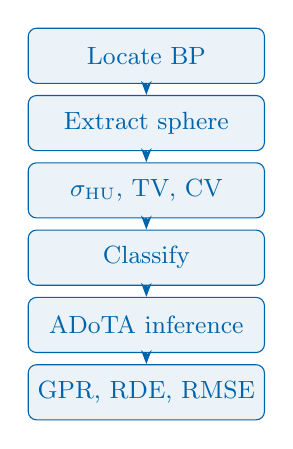
\begin{tikzpicture}[
          box/.style={draw=tudelft, rounded corners=3pt,
                      minimum width=3cm, minimum height=0.7cm,
                      font=\small, text=tudelft, fill=tudelft!8},
          arr/.style={-{Stealth[length=5pt]}, thick, tudelft}
        ]
          \node[box] (bp) {Locate BP};
          \node[box, below=4pt of bp] (sphere) {Extract sphere};
          \node[box, below=4pt of sphere] (met) {$\sigma_{\text{HU}}$, TV, CV};
          \node[box, below=4pt of met] (cls) {Classify};
          \node[box, below=4pt of cls] (inf) {ADoTA inference};
          \node[box, below=4pt of inf] (eval) {GPR, RDE, RMSE};
          \draw[arr] (bp) -- (sphere);
          \draw[arr] (sphere) -- (met);
          \draw[arr] (met) -- (cls);
          \draw[arr] (cls) -- (inf);
          \draw[arr] (inf) -- (eval);
        \end{tikzpicture}
      \end{center}
    \end{column}
  \end{columns}
\end{frame}

\begin{frame}{Heterogeneity Metrics}
  Let $\mathbf{v} = \{v_1, \ldots, v_N\}$ be the set of HU values inside the
  spherical neighbourhood of radius~$r$ around the Bragg peak.

  \vspace{8pt}
  \begin{columns}[T]
    \begin{column}{0.32\textwidth}
      \centering
      \textbf{Standard deviation}\\[4pt]
      $\displaystyle \sigma_{\text{HU}} = \sqrt{\frac{1}{N}\sum_{i=1}^{N}(v_i - \bar{v})^2}$
      \\[6pt]
      {\small Used as the classification criterion.}
    \end{column}
    \begin{column}{0.32\textwidth}
      \centering
      \textbf{Total Variation}\\[4pt]
      $\displaystyle \text{TV} = \sum_{i=1}^{N-1} |v_{i+1} - v_i|$
      \\[6pt]
      {\small Measures roughness /\\local density jumps.}
    \end{column}
    \begin{column}{0.32\textwidth}
      \centering
      \textbf{Coeff.\ of Variation}\\[4pt]
      $\displaystyle \text{CV} = \frac{\sigma(\mathbf{v})}{|\mu(\mathbf{v})|}$
      \\[6pt]
      {\small Relative spread of\\tissue density.}
    \end{column}
  \end{columns}

  \vspace{10pt}
  \begin{block}{Classification rule}
    A beamlet is labelled \textbf{interface} if
    $\sigma_{\text{HU}} > \tau$, and \textbf{homogeneous} otherwise.
    Both experiments use $\tau = \SI{200}{HU}$.
  \end{block}
\end{frame}

\begin{frame}{Performance Metrics}
  Four dose-prediction quality metrics are evaluated per beamlet:

  \vspace{6pt}
  \begin{columns}[T]
    \begin{column}{0.48\textwidth}
      \textbf{Gamma Pass Rate (GPR)}
      \begin{itemize}
        \item $\gamma(2\%/\SI{2}{mm})$, lower dose cutoff \SI{10}{\percent}
        \item Global gamma; values in \SI{}{\percent}
        \item Industry-standard composite metric
      \end{itemize}

      \vspace{8pt}
      \textbf{Relative Dose Error (RDE)}
      \begin{itemize}
        \item $\displaystyle \text{RDE} = \frac{|D_{\max}^{\text{pred}} - D_{\max}^{\text{ref}}|}{D_{\max}^{\text{ref}}} \times 100\%$
        \item Clinically relevant: captures peak-dose mismatch
      \end{itemize}
    \end{column}

    \begin{column}{0.48\textwidth}
      \textbf{Root Mean Square Error (RMSE)}
      \begin{itemize}
        \item Computed over the full 3-D dose grid in Gy
        \item Absolute measure of voxel-wise deviation
      \end{itemize}

      \vspace{8pt}
      \textbf{Mean Absolute Percentage Error (MAPE)}
      \begin{itemize}
        \item Applied to voxels with dose $> 10\%$ of the maximum
        \item Relative accuracy in the high-dose region
      \end{itemize}
    \end{column}
  \end{columns}
\end{frame}

% ════════════════════════════════════════════════════════════
\section{Experimental Setup}
% ════════════════════════════════════════════════════════════

\begin{frame}{Experimental Setup}
  \begin{columns}[T]
    \begin{column}{0.48\textwidth}
      \textbf{Common parameters:}
      \begin{itemize}
        \item \textbf{Model}: DoTA3D\_v3 (grid search v11)
        \item \textbf{Dataset}: pelvis single-Gaussian,\\
              69\,295 beamlets after exclusions\\
              (\SI{70}{MeV}--\SI{250}{MeV})
        \item \textbf{Grid}: $160 \times 30 \times 30$ voxels\\
              at $\SI{2}{mm}$ isotropic resolution
        \item \textbf{Threshold}: $\tau = \SI{200}{HU}$
        \item \textbf{GPR}: $\gamma(2\%/\SI{2}{mm})$
      \end{itemize}
    \end{column}

    \begin{column}{0.48\textwidth}
      \textbf{Variable: sphere radius $r$}
      \vspace{4pt}
      \begin{table}[h]
        \centering
        \small
        \begin{tabular}{lcc}
          \toprule
          & \textbf{Exp.~1} & \textbf{Exp.~2} \\
          \midrule
          Radius $r$    & \SI{10}{mm} & \SI{5}{mm}  \\
          Run date      & 1 Apr       & 7 Apr       \\
          Runtime       & $\sim$23\,h & $\sim$23\,h \\
          \bottomrule
        \end{tabular}
      \end{table}

      \vspace{8pt}
      {\small \textbf{Rationale}: the radius defines how much tissue
       context surrounds the Bragg peak.  A larger sphere captures
       more distant heterogeneities; a smaller sphere focuses on the
       immediate dosimetric neighbourhood.}
    \end{column}
  \end{columns}
\end{frame}

% ════════════════════════════════════════════════════════════
\section{Results}
% ════════════════════════════════════════════════════════════

% ── Prevalence ──────────────────────────────────────────────
\begin{frame}{Prevalence of Interface Beamlets}
  \begin{table}
    \centering
    \begin{tabular}{lccccc}
      \toprule
      & \textbf{Total} & \multicolumn{2}{c}{\textbf{Homogeneous}} &
        \multicolumn{2}{c}{\textbf{Interface}} \\
      \cmidrule(lr){3-4}\cmidrule(lr){5-6}
      & & $N$ & \% & $N$ & \% \\
      \midrule
      $r = \SI{10}{mm}$ & 69\,295 & 41\,547 & 60.0 & 27\,748 & 40.0 \\
      $r = \SI{5}{mm}$  & 69\,295 & 52\,305 & 75.5 & 16\,990 & 24.5 \\
      \bottomrule
    \end{tabular}
  \end{table}

  \vspace{6pt}
  \begin{itemize}
    \item Reducing the radius from \SI{10}{mm} to \SI{5}{mm}
          \textbf{decreases interface prevalence from 40\% to 24.5\%}.
    \item At $r = \SI{5}{mm}$ the sphere contains $\sim$65 voxels
          vs.\ $\sim$524 voxels at $r = \SI{10}{mm}$ —
          a smaller window is more selective.
    \item In either case, a \emph{substantial fraction} of training beamlets
          traverse a tissue boundary.
  \end{itemize}
\end{frame}

% ── Performance comparison ──────────────────────────────────
\begin{frame}{Performance: Interface vs.\ Homogeneous}
  \begin{table}
    \centering\small
    \begin{tabular}{llcccc}
      \toprule
      \textbf{Exp.} & \textbf{Group} & \textbf{GPR [\%]} & \textbf{MAPE [\%]}
        & \textbf{RDE [\%]} & \textbf{RMSE [Gy]} \\
      \midrule
      \multirow{2}{*}{$r{=}\SI{10}{mm}$}
        & Homogeneous & $99.11 \pm 1.23$ & $5.11 \pm 1.63$ & $0.146 \pm 0.081$ & $(8.9 \pm 3.8) \times 10^{-6}$ \\
        & Interface   & $98.41 \pm 1.68$ & $6.12 \pm 2.09$ & $0.192 \pm 0.078$ & $(10.7 \pm 5.2) \times 10^{-6}$ \\
      \midrule
      \multirow{2}{*}{$r{=}\SI{5}{mm}$}
        & Homogeneous & $98.99 \pm 1.30$ & $5.28 \pm 1.71$ & $0.154 \pm 0.082$ & $(9.1 \pm 3.9) \times 10^{-6}$ \\
        & Interface   & $98.33 \pm 1.82$ & $6.22 \pm 2.22$ & $0.196 \pm 0.079$ & $(11.0 \pm 5.6) \times 10^{-6}$ \\
      \bottomrule
    \end{tabular}
  \end{table}

  \vspace{6pt}
  \begin{columns}[T]
    \begin{column}{0.48\textwidth}
      \textbf{Key observations:}
      \begin{itemize}
        \item Interface beamlets show consistently \textbf{worse} performance
              across all four metrics in both experiments.
        \item GPR gap: $\sim$\SI{0.7}{pp} ($r{=}\SI{10}{mm}$),
              $\sim$\SI{0.66}{pp} ($r{=}\SI{5}{mm}$).
        \item RDE gap: $\sim$32\% relative increase at interfaces.
      \end{itemize}
    \end{column}
    \begin{column}{0.48\textwidth}
      \textbf{Radius effect:}
      \begin{itemize}
        \item The performance \emph{gap} is similar for both radii,
              suggesting the degradation is robust and not an artefact
              of neighbourhood size.
        \item A smaller radius produces a more selective (purer) interface
              class — but the effect magnitude is preserved.
      \end{itemize}
    \end{column}
  \end{columns}
\end{frame}

% ── Violin plots ────────────────────────────────────────────
\begin{frame}{Metric Distributions — $r = \SI{10}{mm}$}
  \begin{center}
    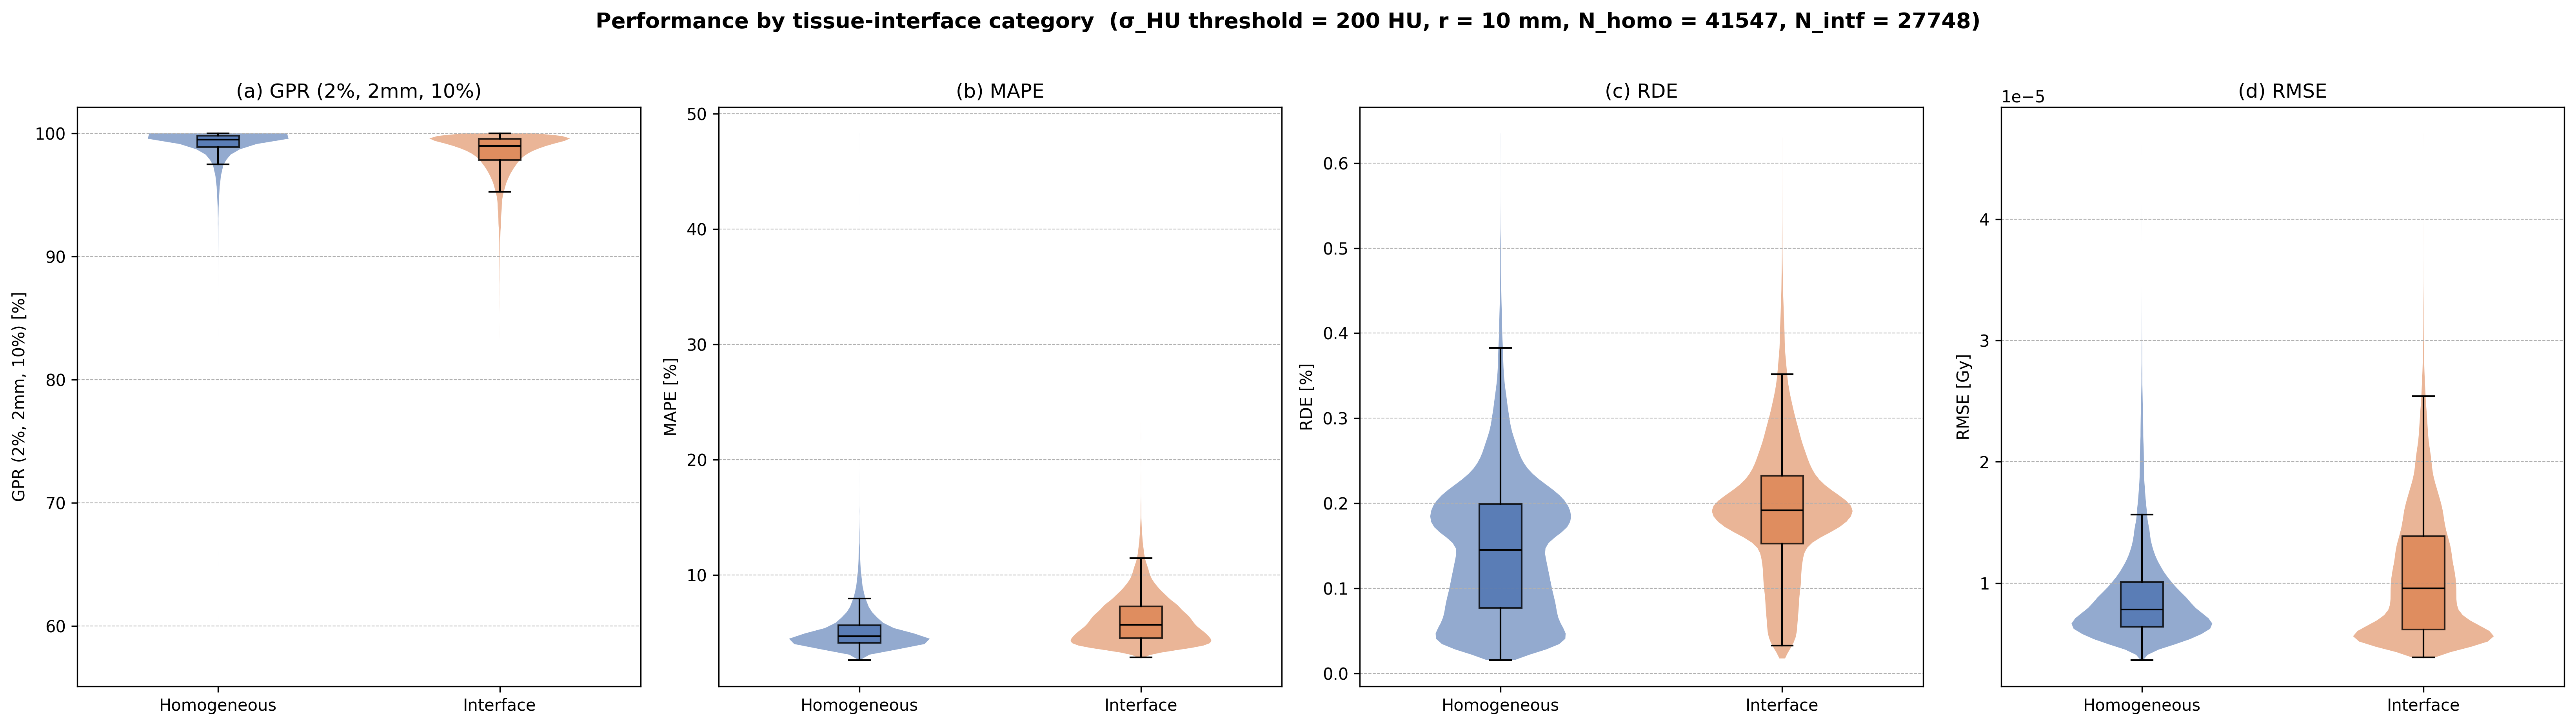
\includegraphics[width=0.92\textwidth]{run1_r10mm/interface_vs_homogeneous_violin.png}
  \end{center}
  \vspace{-4pt}
  {\small Violin + box plots of GPR, MAPE, RDE, and RMSE split by
   tissue class.  Interface beamlets (orange) exhibit heavier tails
   towards worse performance.}
\end{frame}

\begin{frame}{Metric Distributions — $r = \SI{5}{mm}$}
  \begin{center}
    
\includegraphics[width=0.92\textwidth]{run2_r5mm/interface_vs_homogeneous_violin.png}
  \end{center}
  \vspace{-4pt}
  {\small Same violin layout for the smaller neighbourhood.  The
   distributions are qualitatively similar; the interface class has a
   slightly more pronounced tail due to higher classification purity.}
\end{frame}

% ── Histograms ──────────────────────────────────────────────
\begin{frame}{$\sigma_{\text{HU}}$ Distribution}
  \begin{columns}
    \begin{column}{0.48\textwidth}
      \centering
      \textbf{$r = \SI{10}{mm}$}\\[4pt]
      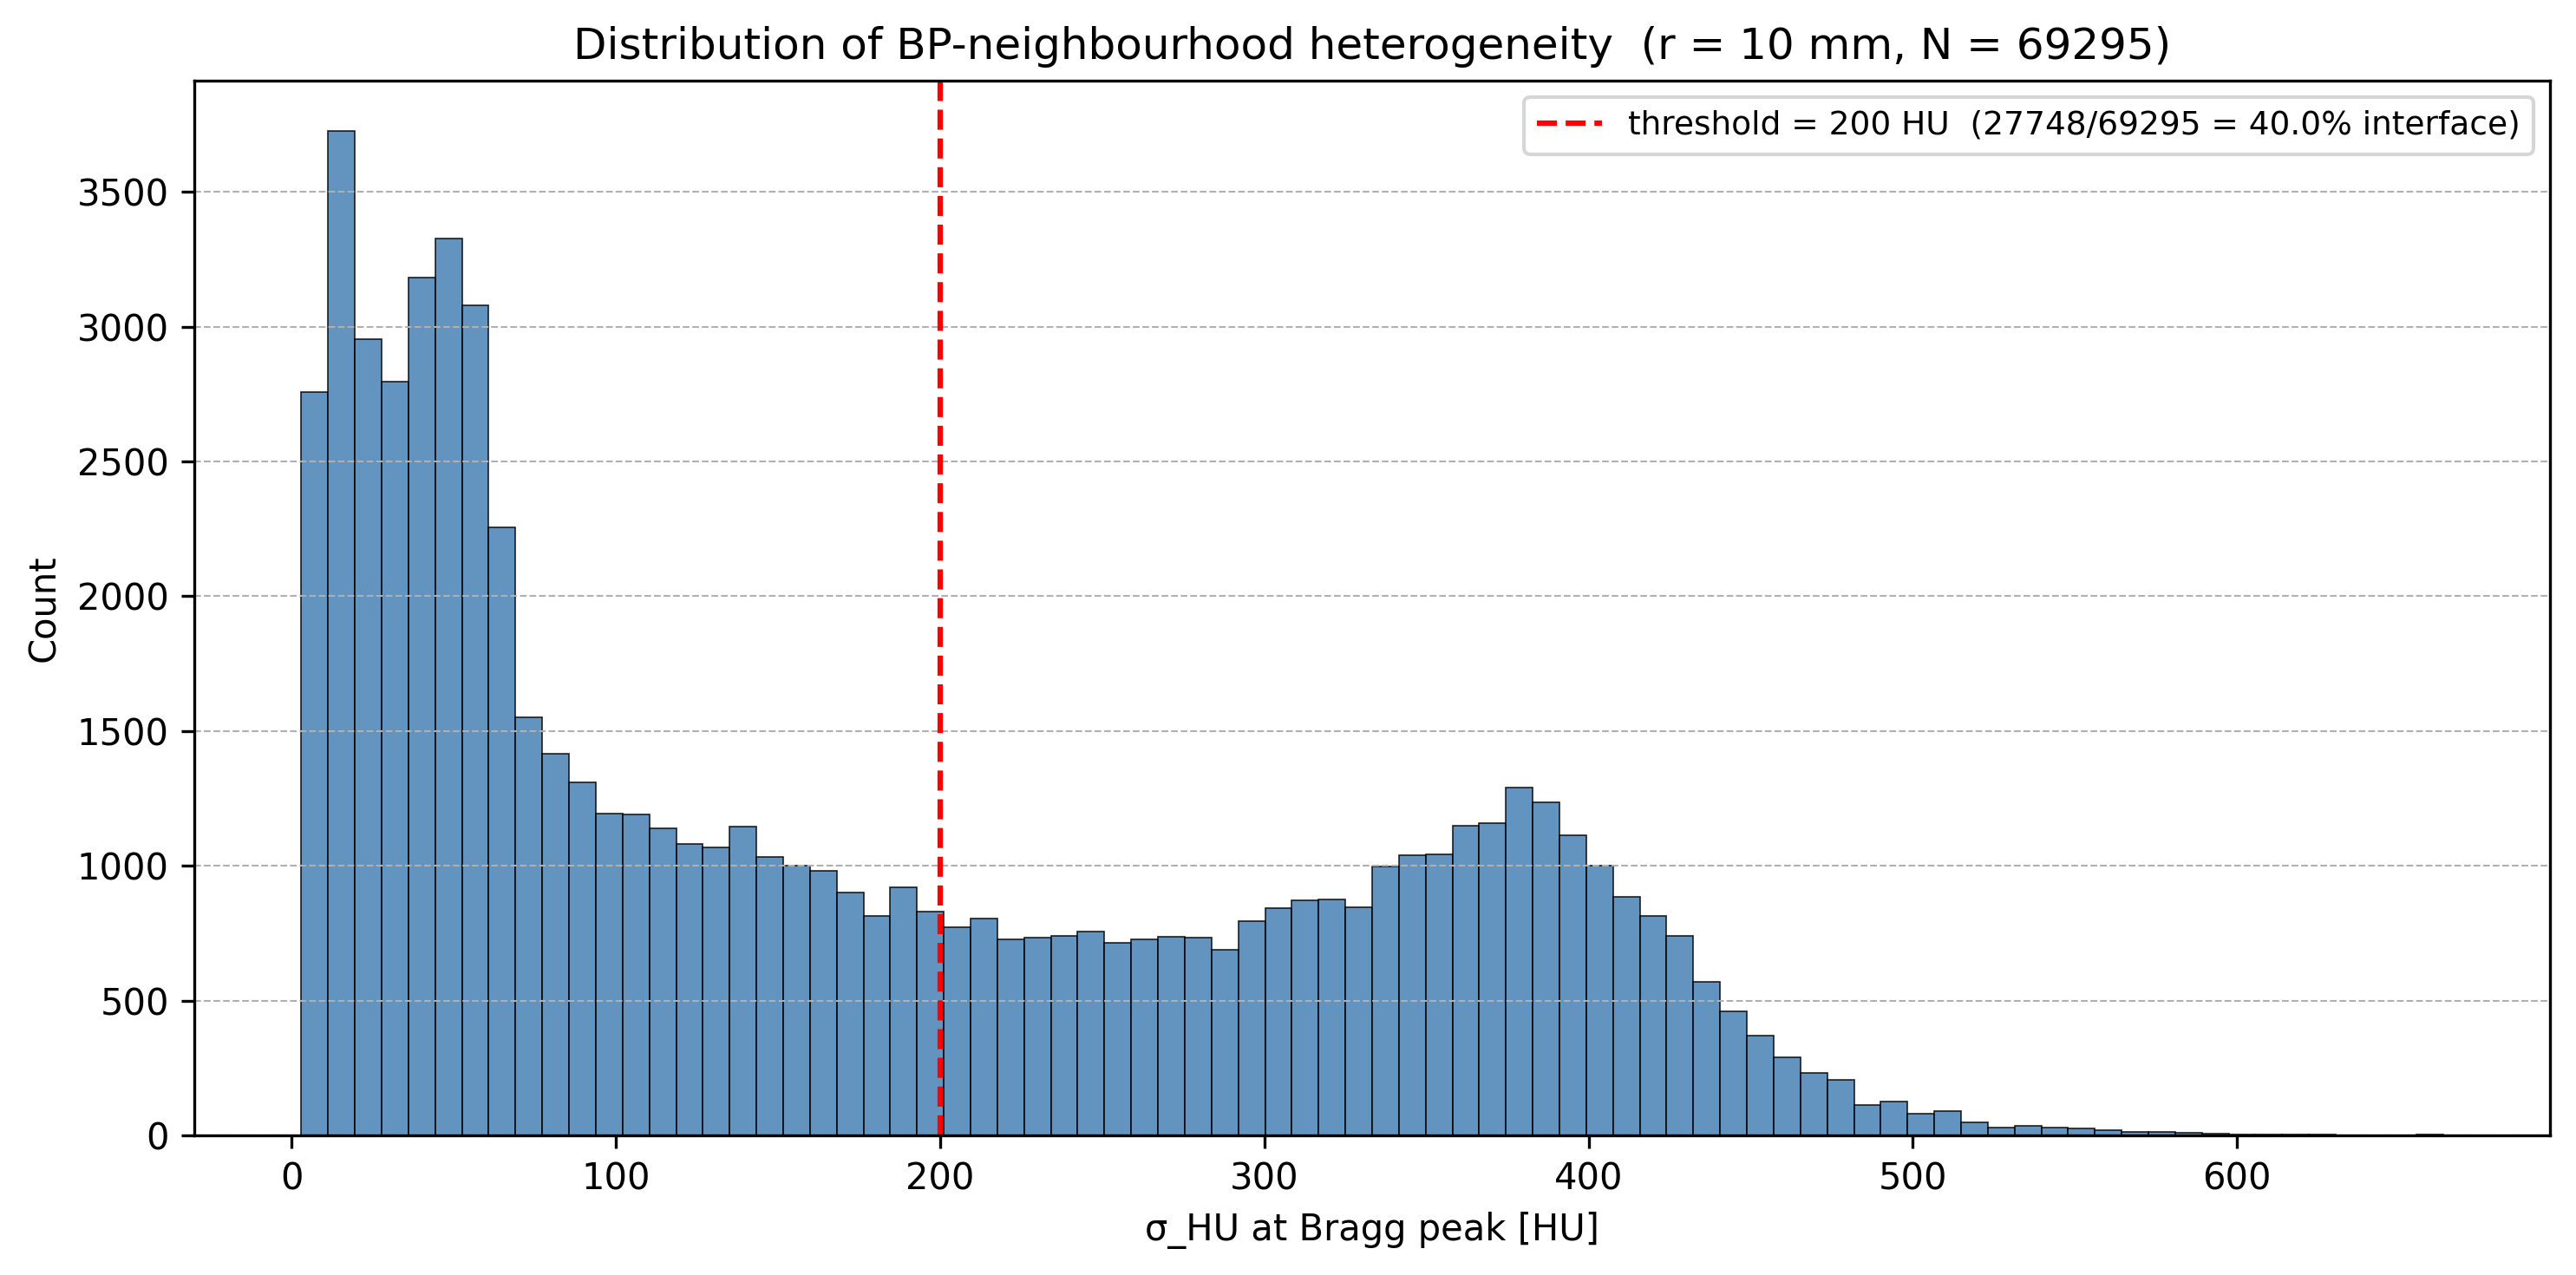
\includegraphics[width=\textwidth]{run1_r10mm/sigma_hu_histogram.png}
    \end{column}
    \begin{column}{0.48\textwidth}
      \centering
      \textbf{$r = \SI{5}{mm}$}\\[4pt]
      
\includegraphics[width=\textwidth]{run2_r5mm/sigma_hu_histogram.png}
    \end{column}
  \end{columns}

  \vspace{6pt}
  {\small The threshold $\tau = \SI{200}{HU}$ (dashed line) sits in the
   valley between the two modes.  The larger sphere produces a broader
   distribution, as distant voxels contribute additional variance.}
\end{frame}

% ── Scatter: σ_HU vs GPR ───────────────────────────────────
\begin{frame}{$\sigma_{\text{HU}}$ vs.\ Gamma Pass Rate}
  \begin{columns}
    \begin{column}{0.48\textwidth}
      \centering
      \textbf{$r = \SI{10}{mm}$}\\[4pt]
      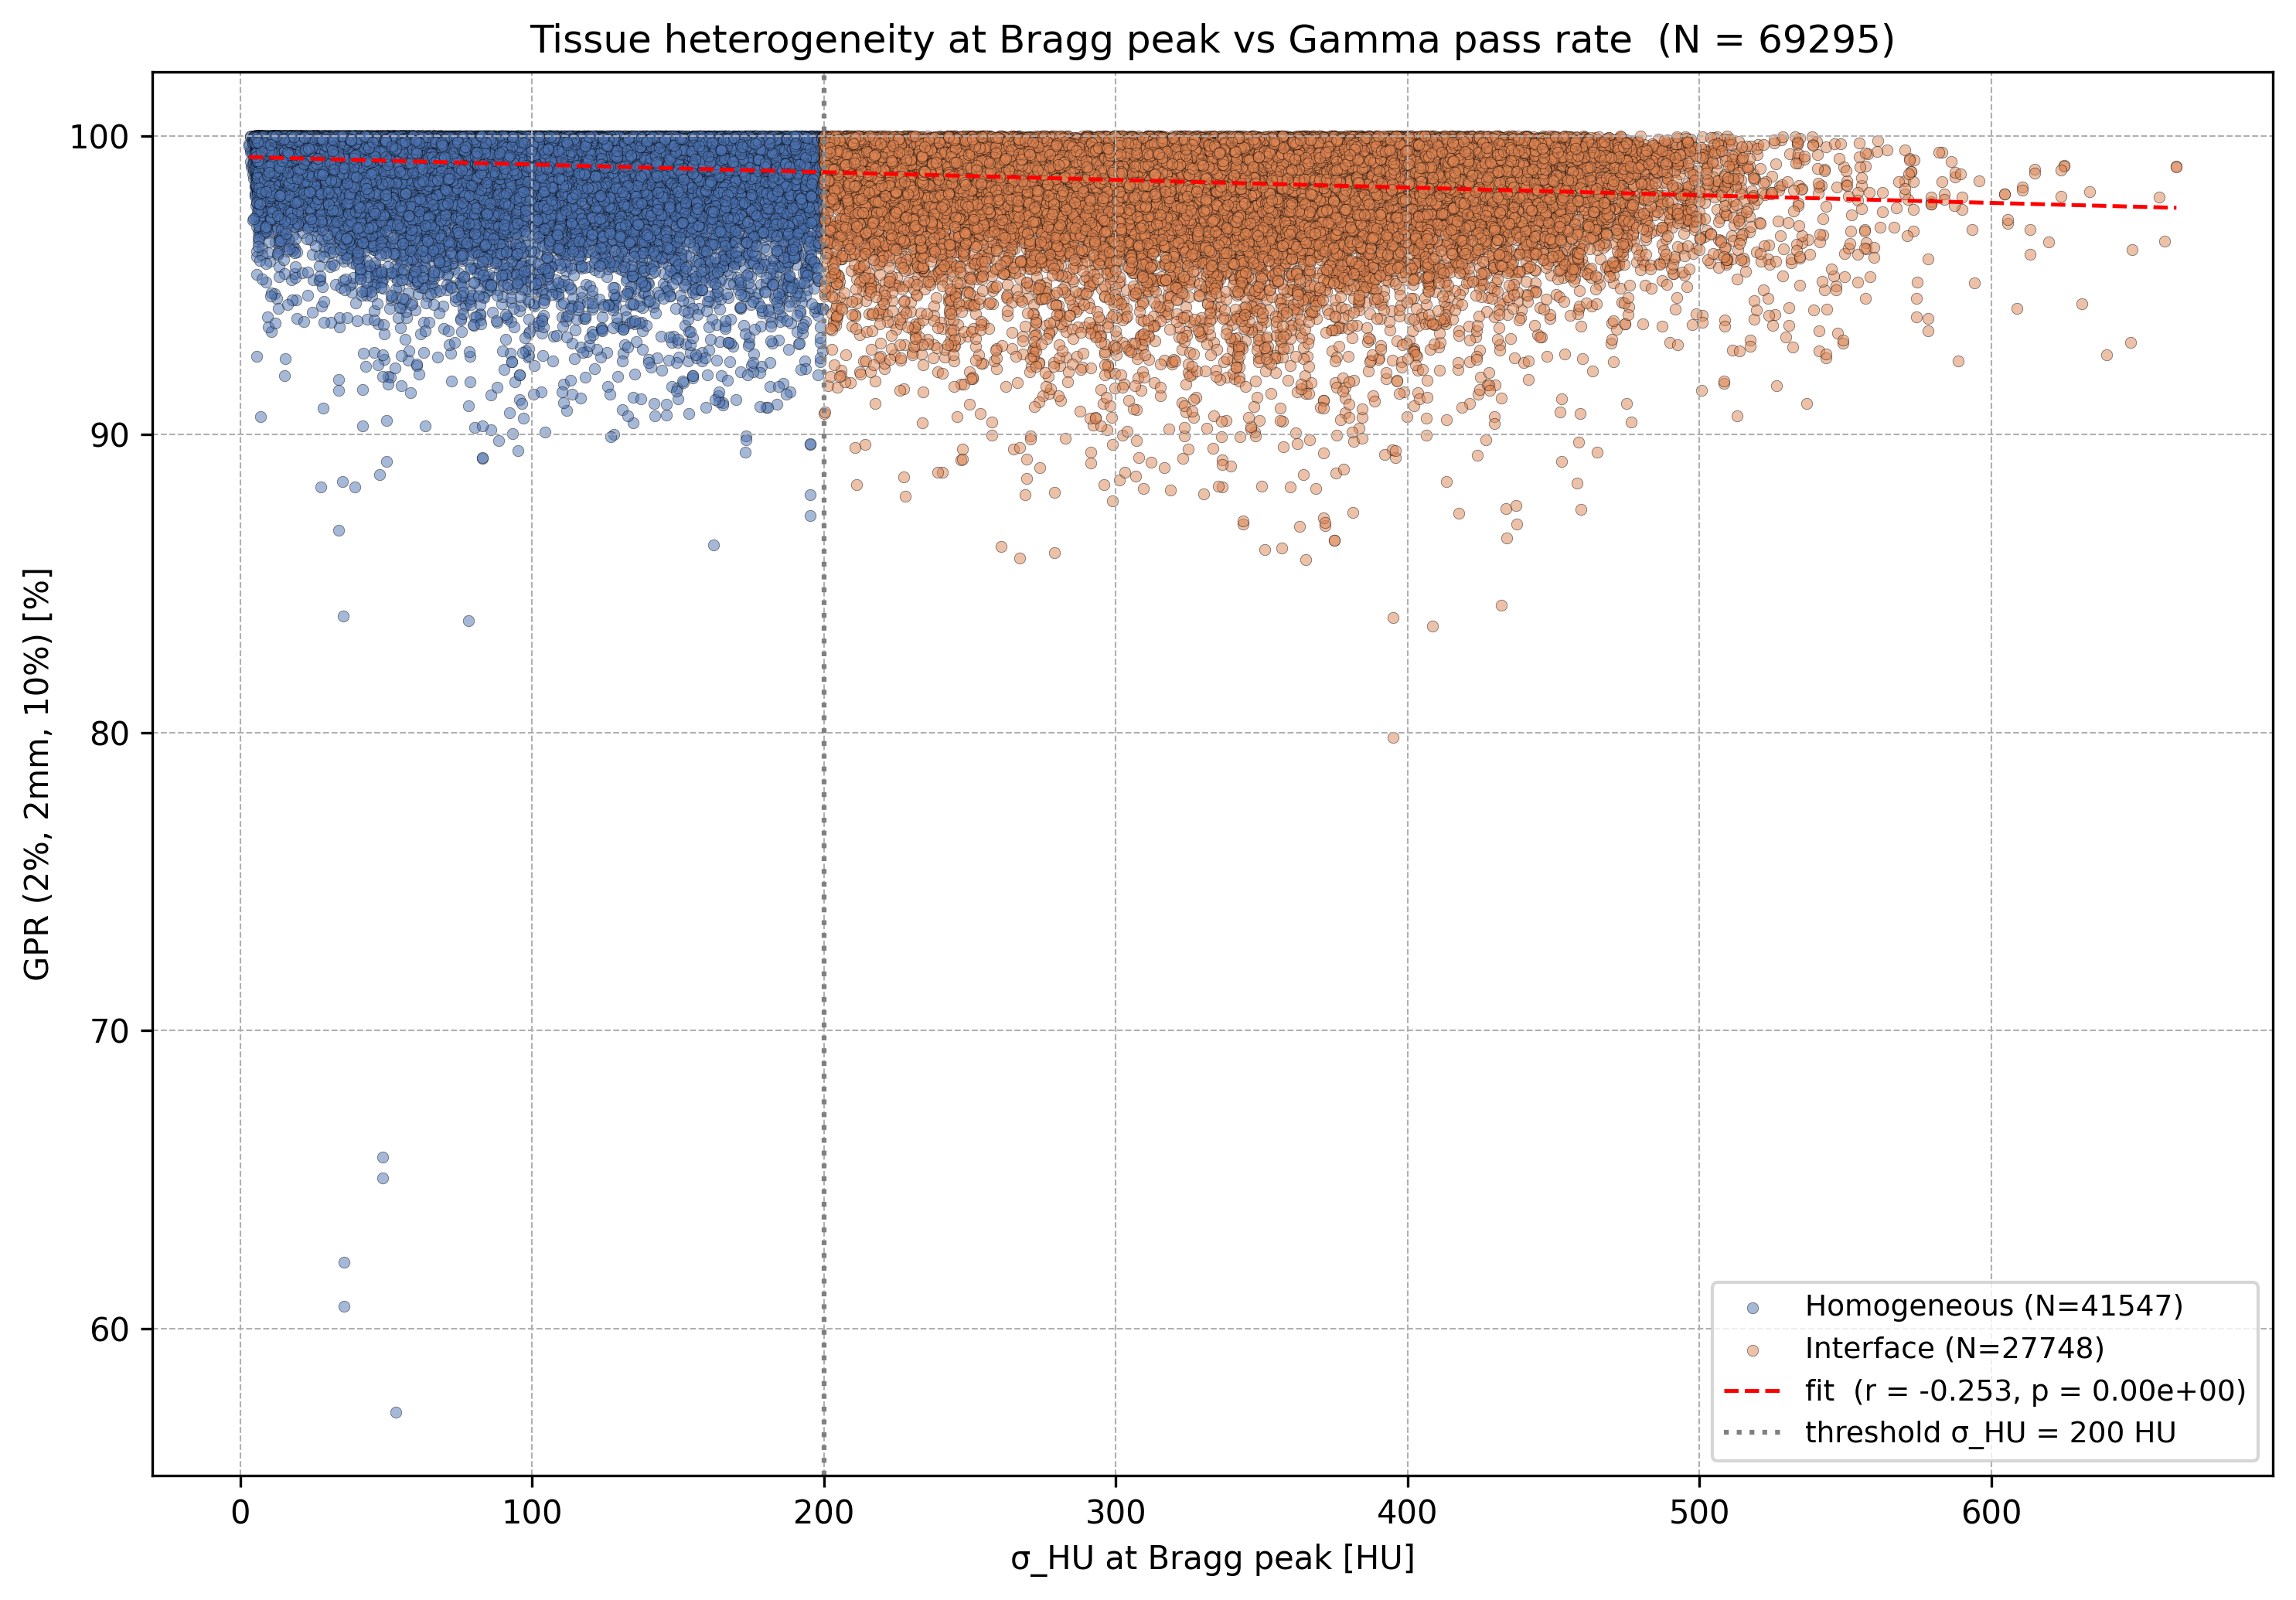
\includegraphics[width=\textwidth]{run1_r10mm/sigma_hu_vs_gpr_scatter.png}
    \end{column}
    \begin{column}{0.48\textwidth}
      \centering
      \textbf{$r = \SI{5}{mm}$}\\[4pt]
      
\includegraphics[width=\textwidth]{run2_r5mm/sigma_hu_vs_gpr_scatter.png}
    \end{column}
  \end{columns}

  \vspace{6pt}
  {\small Higher $\sigma_{\text{HU}}$ is associated with lower GPR.
   The trend is visible in both experiments, confirming that
   tissue heterogeneity around the Bragg peak is a predictor of
   degraded model accuracy.}
\end{frame}

% ── Scatter: TV vs RDE ─────────────────────────────────────
\begin{frame}{Total Variation vs.\ Relative Dose Error}
  \begin{columns}
    \begin{column}{0.48\textwidth}
      \centering
      \textbf{$r = \SI{10}{mm}$}\\[4pt]
      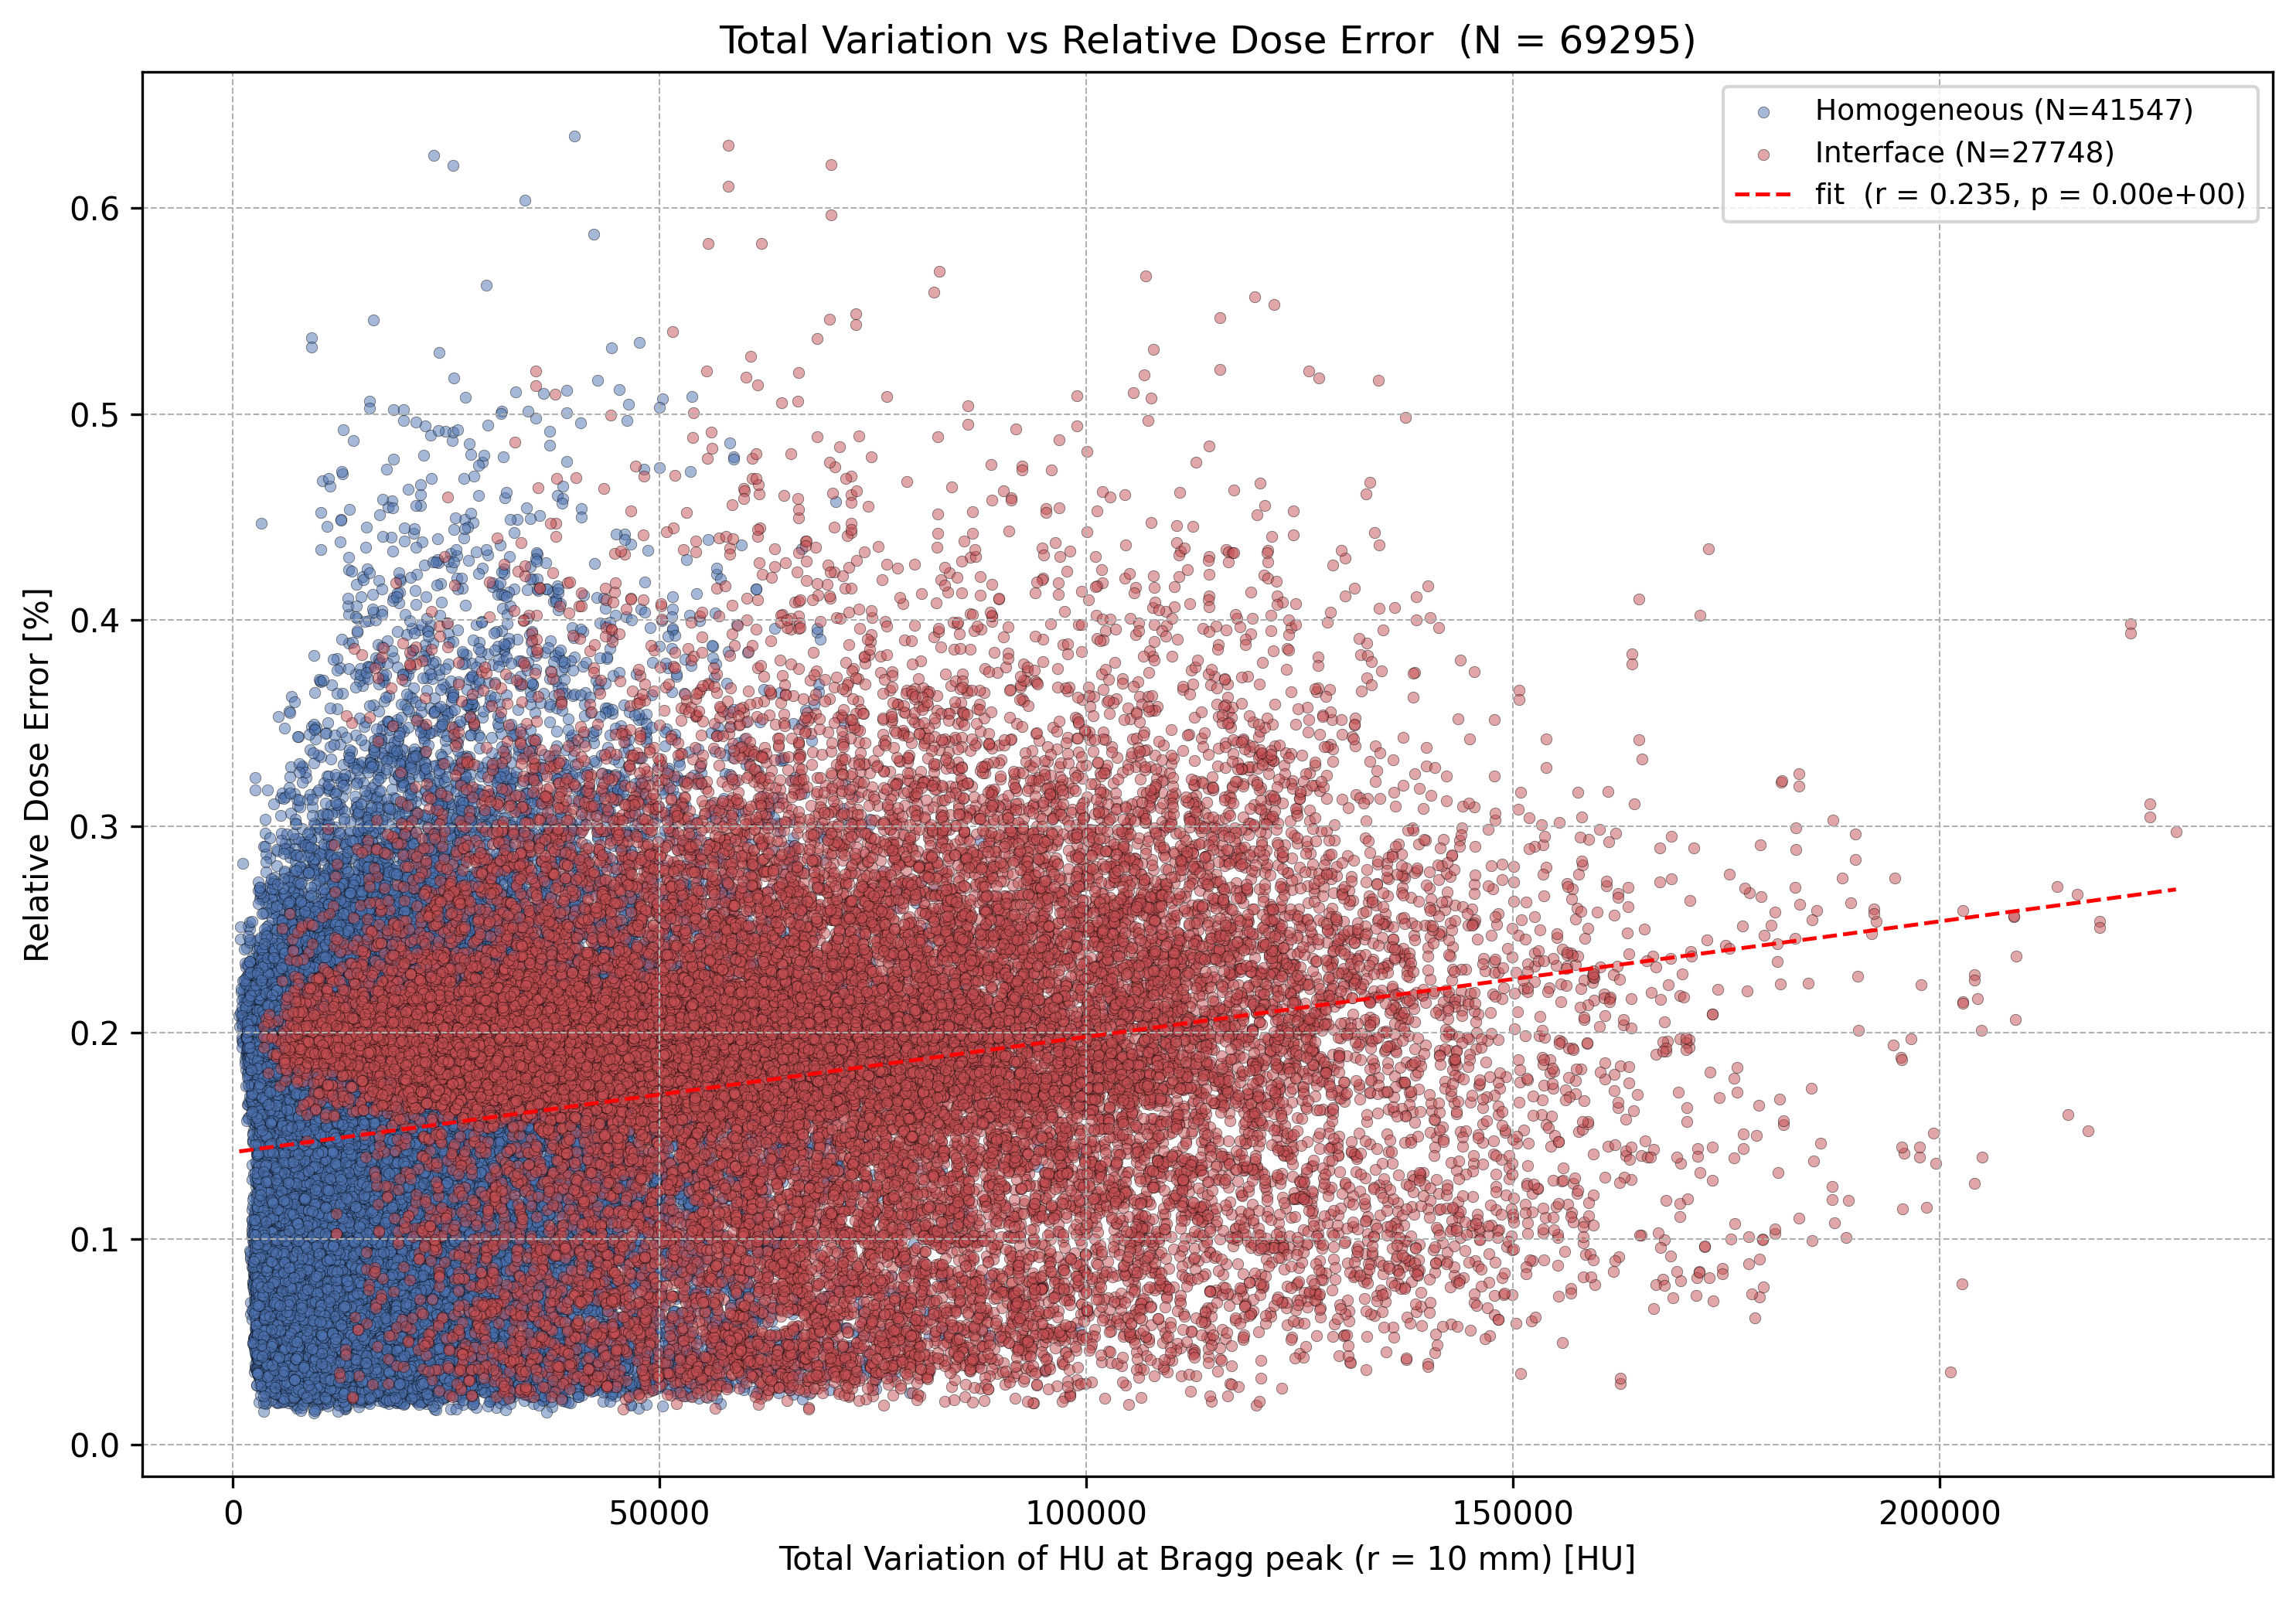
\includegraphics[width=\textwidth]{run1_r10mm/tv_vs_rde_scatter.png}
    \end{column}
    \begin{column}{0.48\textwidth}
      \centering
      \textbf{$r = \SI{5}{mm}$}\\[4pt]
      
\includegraphics[width=\textwidth]{run2_r5mm/tv_vs_rde_scatter.png}
    \end{column}
  \end{columns}

  \vspace{6pt}
  {\small TV captures a complementary view of heterogeneity.  Higher TV
   values correspond to larger RDE, especially in the tail.  The
   TV--RDE correlation supports using multiple texture features for
   error prediction.}
\end{frame}

% ── Scatter: TV vs GPR ─────────────────────────────────────
\begin{frame}{Total Variation vs.\ Gamma Pass Rate}
  \begin{columns}
    \begin{column}{0.48\textwidth}
      \centering
      \textbf{$r = \SI{10}{mm}$}\\[4pt]
      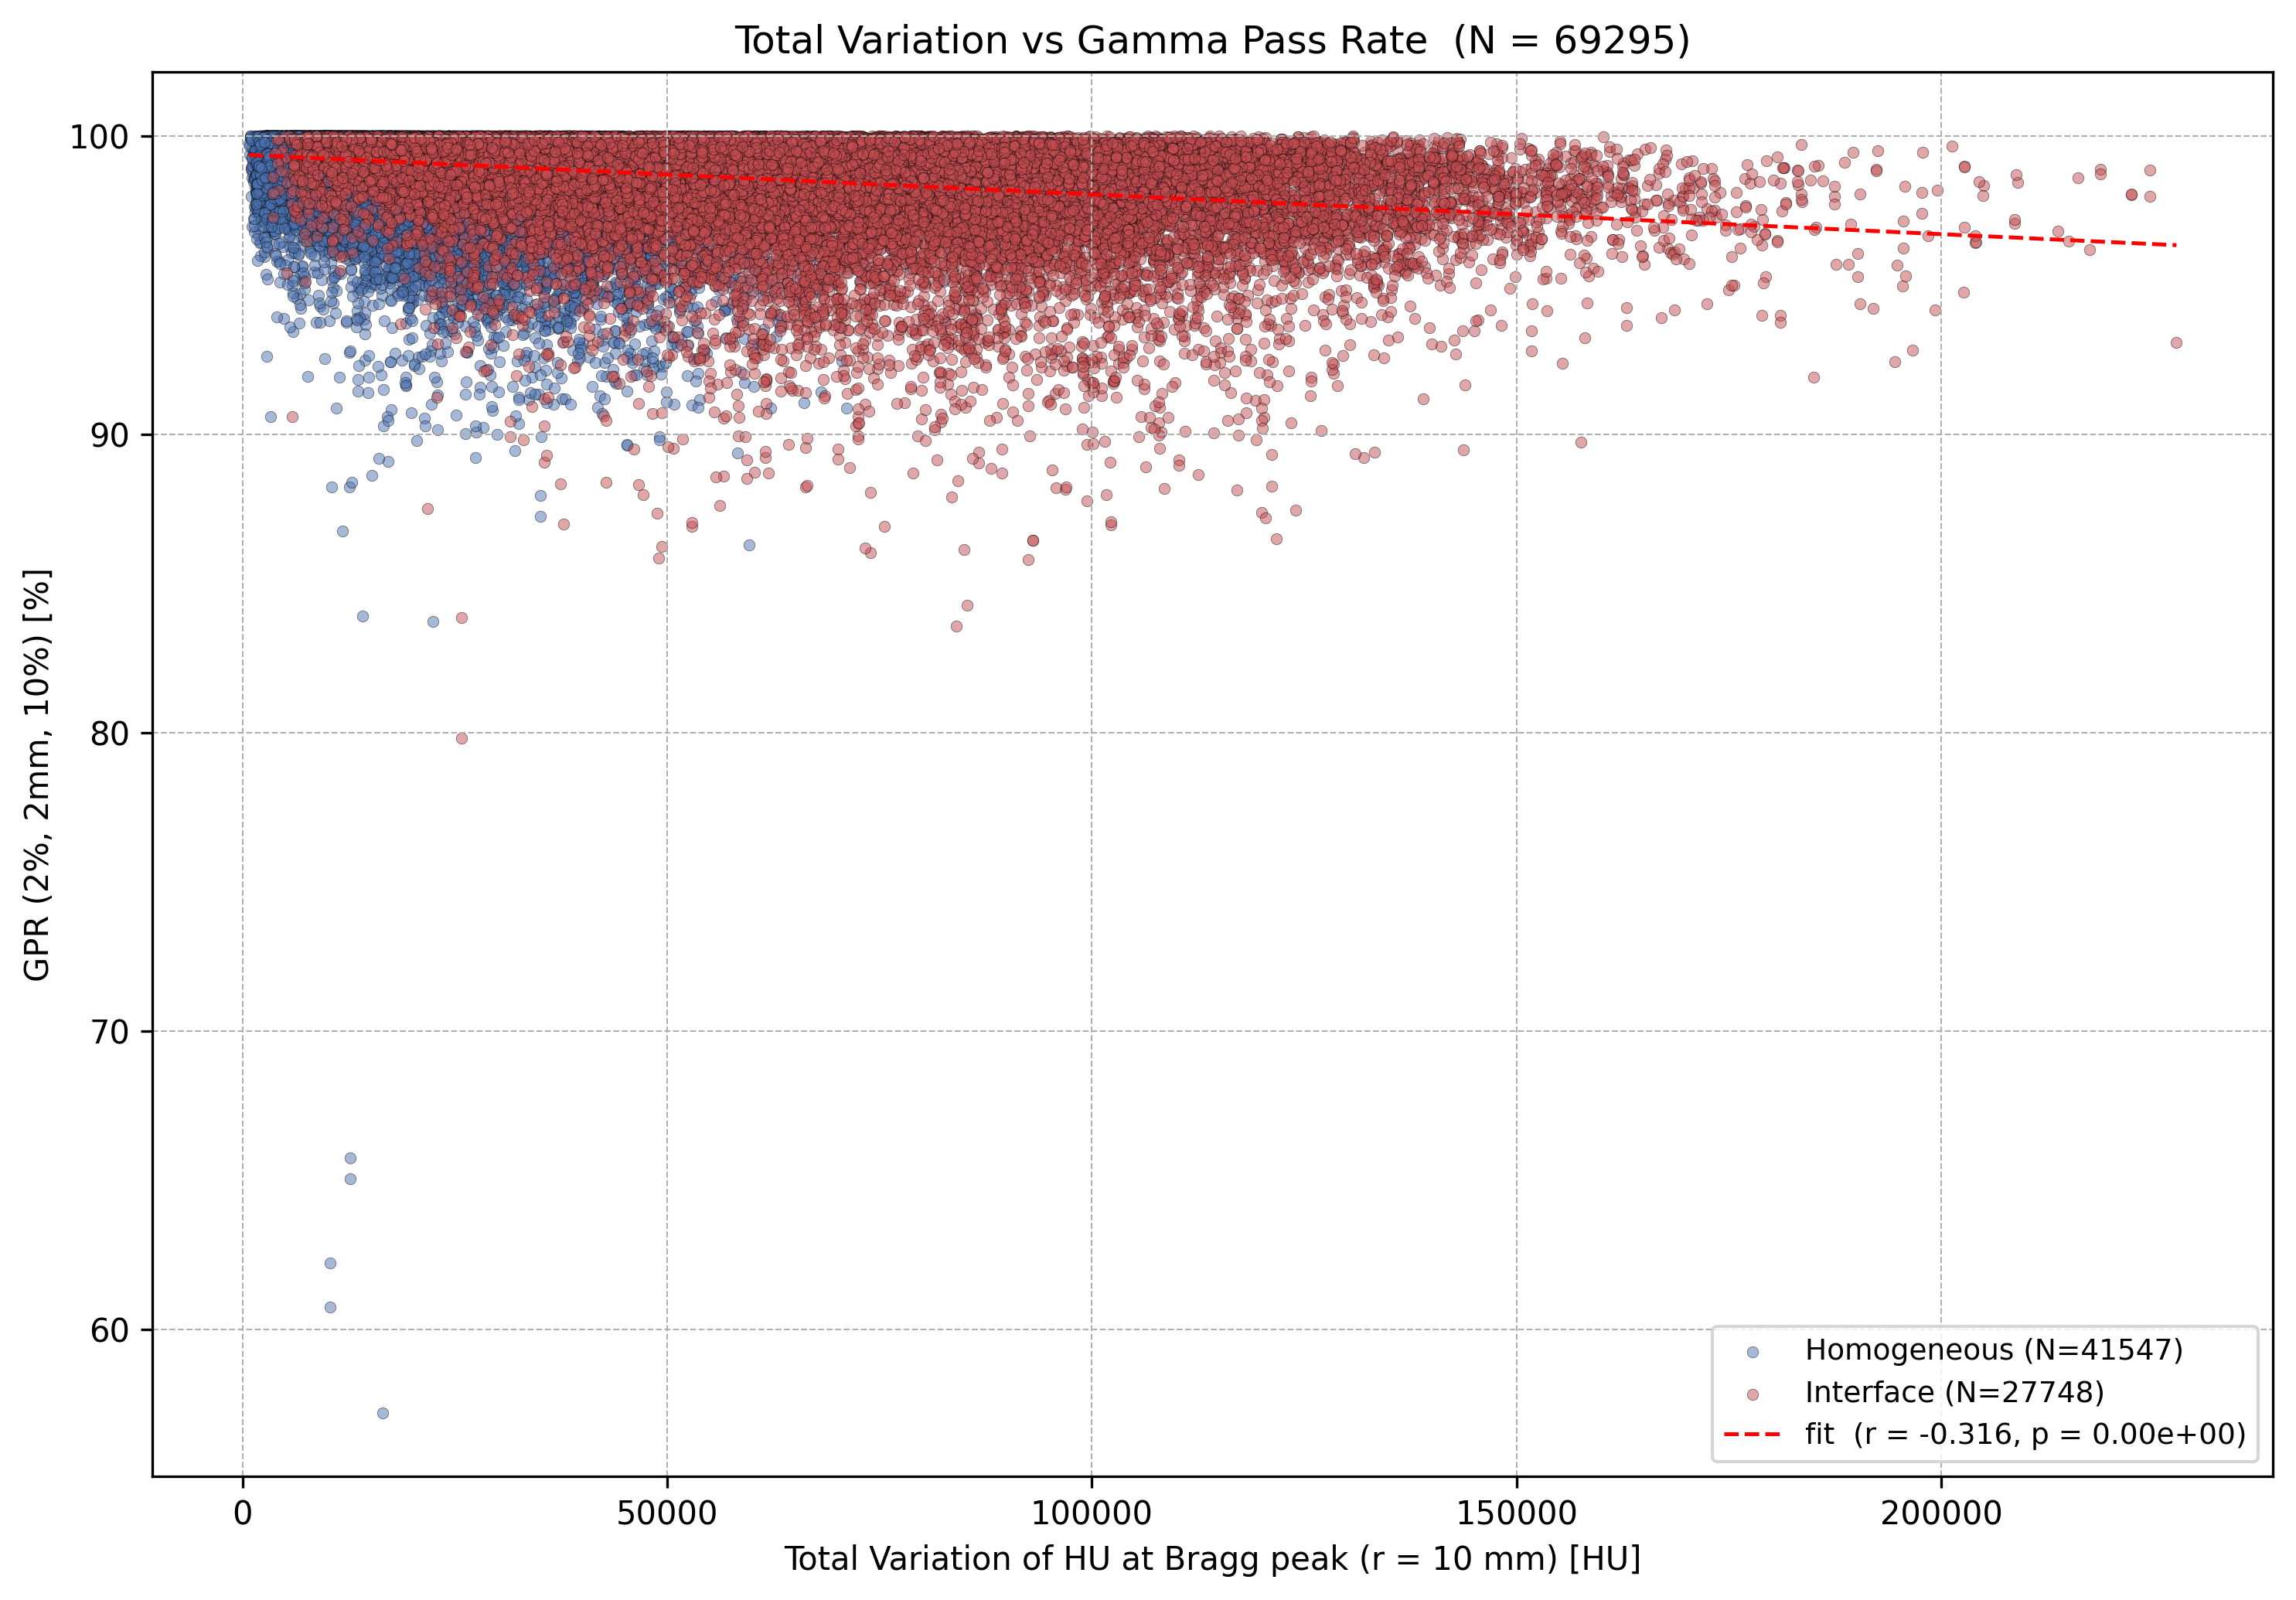
\includegraphics[width=\textwidth]{run1_r10mm/tv_vs_gpr_scatter.png}
    \end{column}
    \begin{column}{0.48\textwidth}
      \centering
      \textbf{$r = \SI{5}{mm}$}\\[4pt]
      
\includegraphics[width=\textwidth]{run2_r5mm/tv_vs_gpr_scatter.png}
    \end{column}
  \end{columns}

  \vspace{6pt}
  {\small Inverse relationship: beamlets with high TV achieve lower GPR.
   This is consistent across both neighbourhood radii.}
\end{frame}

% ════════════════════════════════════════════════════════════
\section{Threshold Sensitivity Sweep}
% ════════════════════════════════════════════════════════════

% ── Problem statement ───────────────────────────────────────
\begin{frame}{Threshold Sweep — Problem Statement}
  \textbf{Motivation:} the previous experiments used a fixed threshold
  $\tau = \SI{200}{HU}$.  A natural question arises:

  \vspace{6pt}
  \begin{block}{Question}
    Is the observed performance gap between interface and homogeneous
    beamlets \textbf{sensitive} to the choice of $\tau$, or does it
    persist across a wide range of thresholds?
  \end{block}

  \vspace{6pt}
  \textbf{Why this matters:}
  \begin{itemize}
    \item If the gap only appears near $\tau = \SI{200}{HU}$, it might
          be an artefact of a particular threshold choice.
    \item If the gap is \textbf{stable across many thresholds}, it
          reflects a genuine, continuous relationship between tissue
          heterogeneity and prediction difficulty.
    \item Understanding the shape of the gap curve informs threshold
          selection for future stratified evaluation and data curation.
  \end{itemize}

  \vspace{6pt}
  \textbf{Experiment:} sweep $\tau$ over $[\SI{50}{HU},\;\SI{400}{HU}]$
  in steps of \SI{10}{HU} (36~values) using the $r = \SI{10}{mm}$ data
  (69\,295~beamlets, pre-computed).
\end{frame}

% ── Mathematical formulation ────────────────────────────────
\begin{frame}{Threshold Sweep — Formulation}
  Given the full set of beamlets $\mathcal{B} = \{b_1, \ldots, b_N\}$, each
  with a pre-computed $\sigma_{\text{HU}}^{(i)}$ and GPR${}^{(i)}$:

  \vspace{6pt}
  For each threshold $\tau \in \{50, 60, \ldots, 400\}$\;HU, define:
  \begin{align*}
    \mathcal{H}(\tau) &= \bigl\{\, b_i \;\big|\; \sigma_{\text{HU}}^{(i)} \le \tau \,\bigr\}
      &&\text{(homogeneous group)} \\[2pt]
    \mathcal{I}(\tau) &= \bigl\{\, b_i \;\big|\; \sigma_{\text{HU}}^{(i)} > \tau \,\bigr\}
      &&\text{(interface group)}
  \end{align*}

  \vspace{2pt}
  The \textbf{GPR gap} at threshold $\tau$ is:
  \[
    \Delta_{\text{GPR}}(\tau)
    = \overline{\text{GPR}}\bigl(\mathcal{H}(\tau)\bigr)
    - \overline{\text{GPR}}\bigl(\mathcal{I}(\tau)\bigr)
  \]

  A positive $\Delta_{\text{GPR}}$ means the interface group has
  \emph{lower} (worse) GPR on average.

  \vspace{6pt}
  Analogous gaps are defined for RDE, MAPE, and RMSE (with the sign
  convention: $\Delta = \text{intf} - \text{homo}$, so a positive value
  means interface is worse).

  \vspace{6pt}
  {\small \textbf{Note}: no model re-inference is needed — the sweep
   re-classifies the same 69\,295 pre-computed beamlets at each $\tau$,
   completing in $< 4$\;seconds.}
\end{frame}

% ── How to read the plots ───────────────────────────────────
\begin{frame}{Threshold Sweep — Reading the Plots}
  Three figures are produced.  Here is how to interpret each one:

  \vspace{4pt}
  \begin{enumerate}
    \item \textbf{GPR Gap vs.\ $\tau$} (dual y-axis):
    \begin{itemize}
      \item \textcolor{red!70!black}{Left axis (red circles)}: $\Delta_{\text{GPR}}(\tau)$ in
            percentage points.  Higher = larger gap.
      \item \textcolor{blue!70!black}{Right axis (blue squares)}: percentage of beamlets
            classified as \emph{interface} at that $\tau$.
      \item As $\tau$ increases, fewer beamlets are labelled interface
            (blue falls), but the selected interface subset becomes
            more extreme.
    \end{itemize}

    \vspace{4pt}
    \item \textbf{Group GPR vs.\ $\tau$}:
    \begin{itemize}
      \item Two curves: mean GPR of the homogeneous group (blue) and the
            interface group (orange).  The \textcolor{red!20!white}{shaded area} between them is the gap.
      \item Shows absolute performance levels, not just the difference.
    \end{itemize}

    \vspace{4pt}
    \item \textbf{All-Metric Gaps} (2$\times$2 panel):
    \begin{itemize}
      \item Extends the analysis to GPR, RDE, MAPE, and RMSE.
      \item Each panel has the same structure: metric gap on the left axis,
            interface prevalence on the right axis.
    \end{itemize}
  \end{enumerate}
\end{frame}

% ── Result: GPR gap vs tau ──────────────────────────────────
\begin{frame}[shrink=5]{GPR Gap vs.\ $\tau$ ($r = \SI{10}{mm}$)}
  \begin{center}
    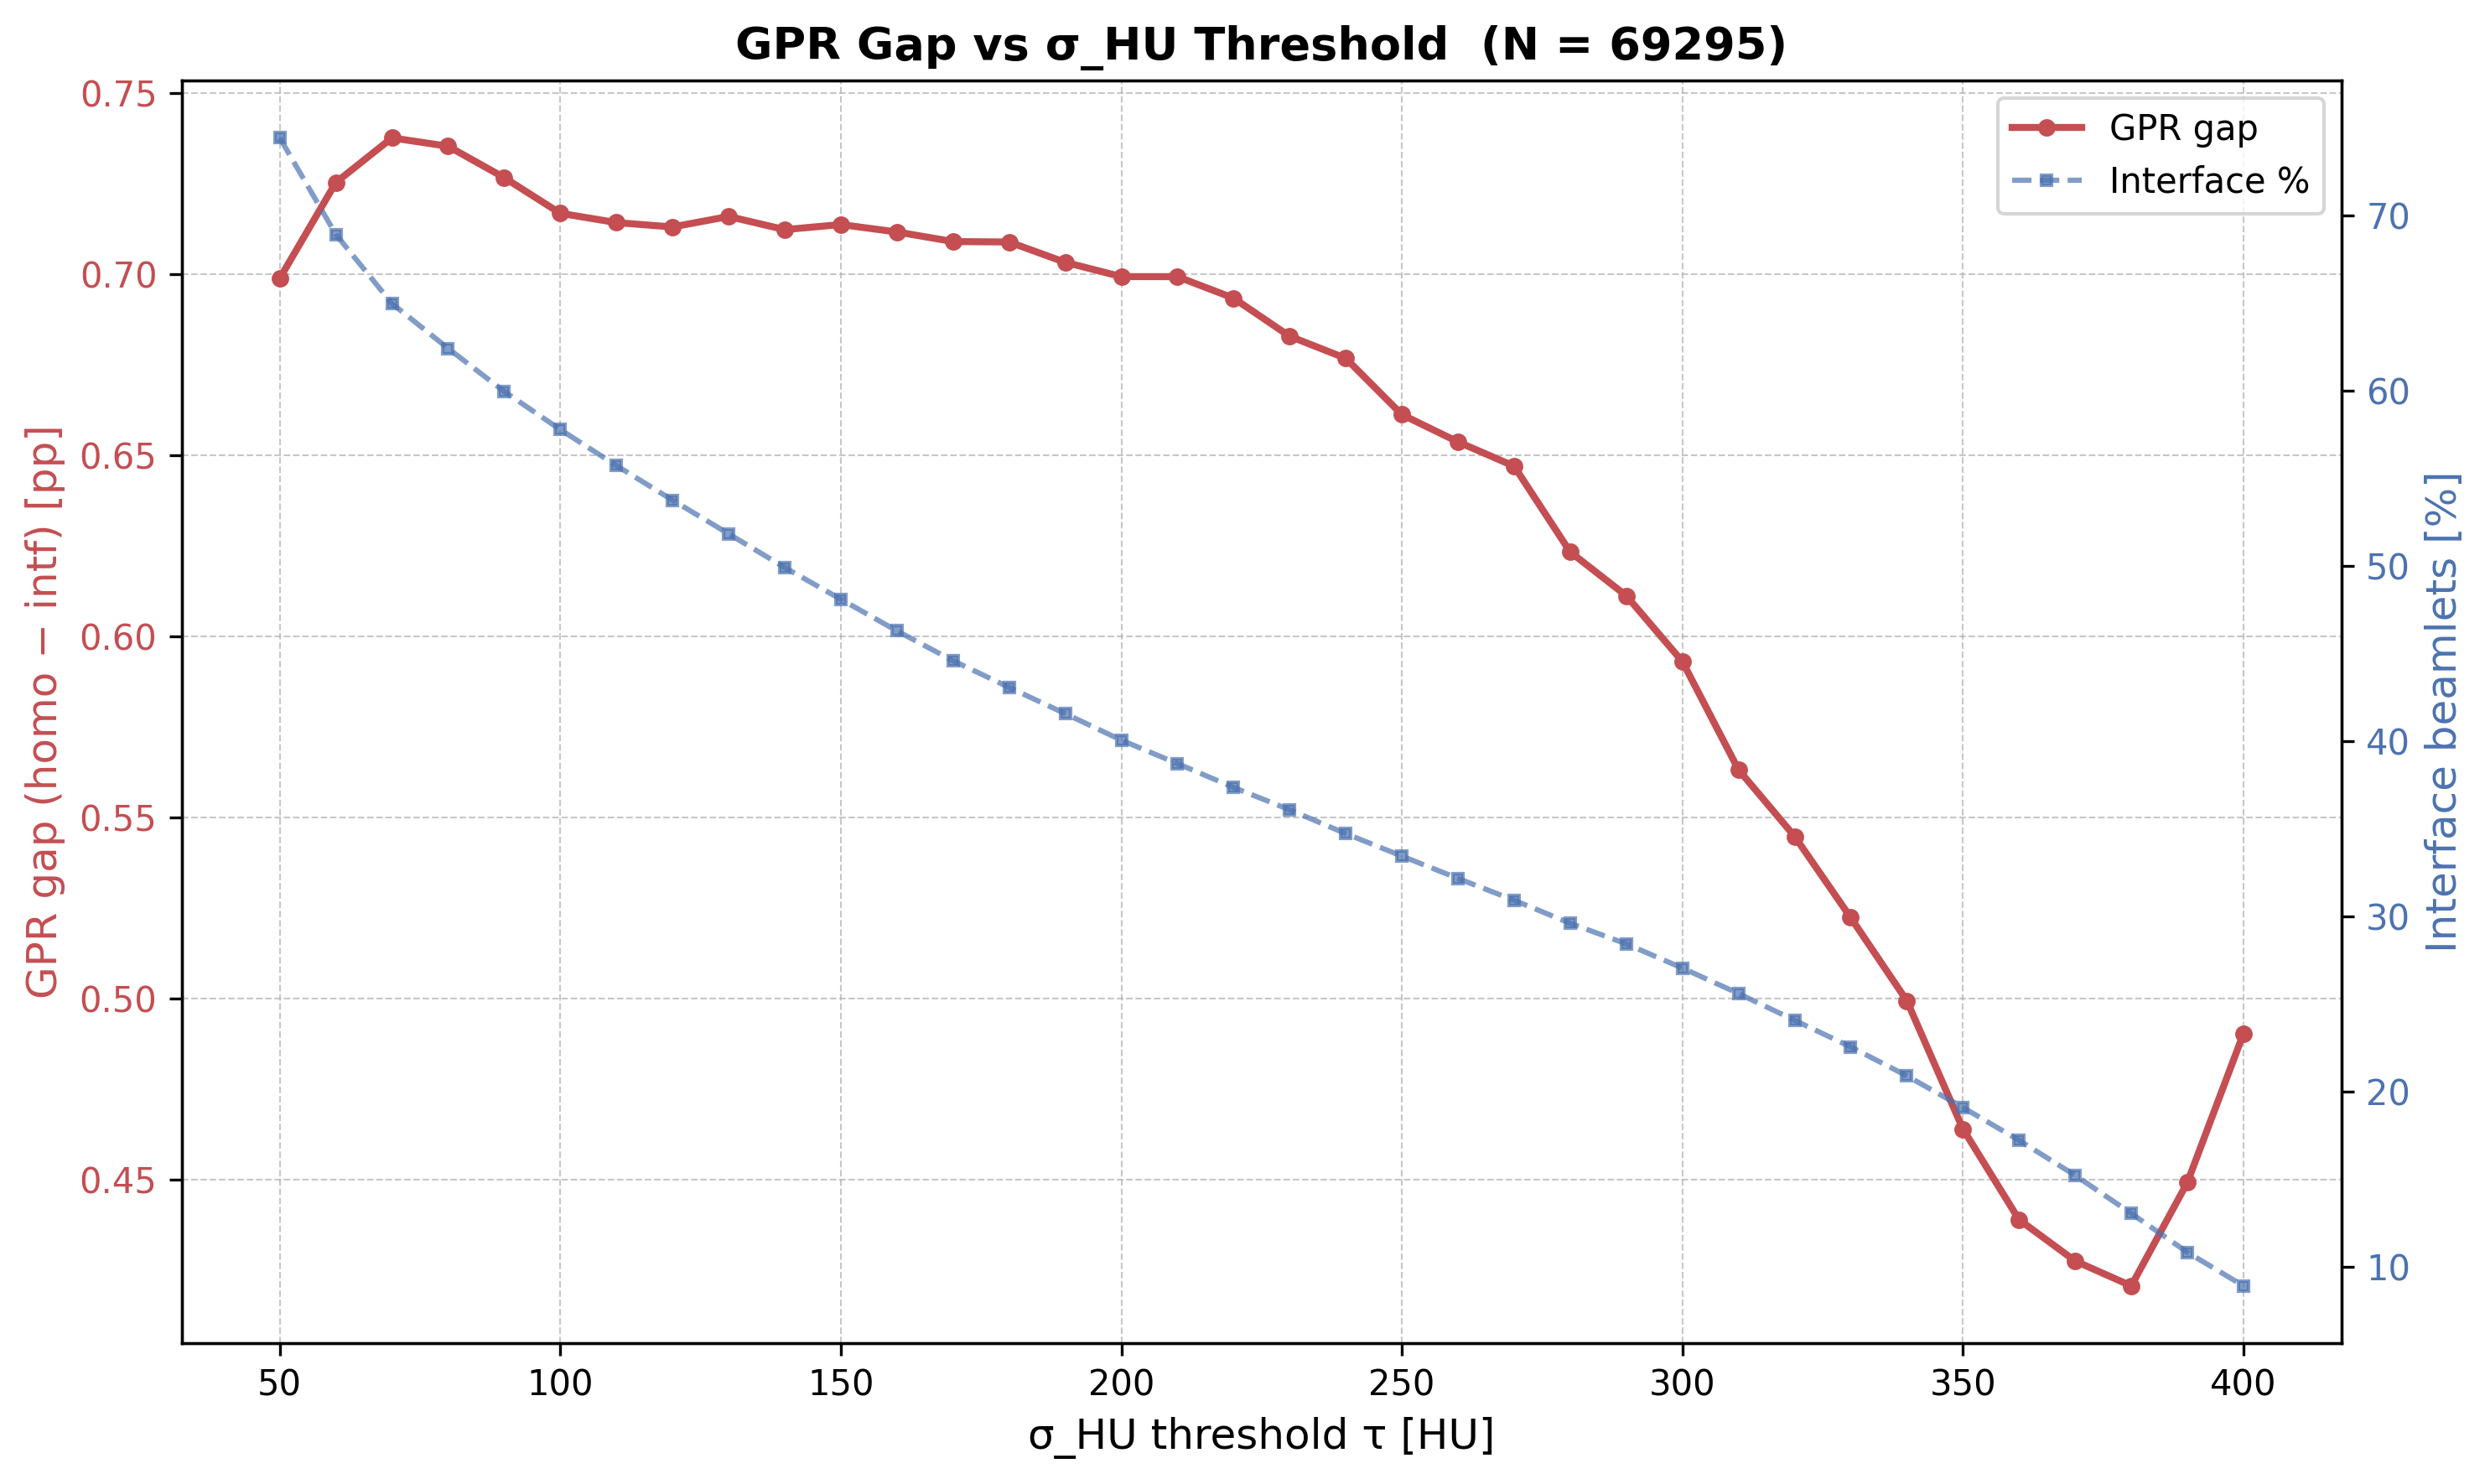
\includegraphics[width=0.68\textwidth]{sweep/gpr_gap_vs_tau.png}
  \end{center}
  \vspace{-4pt}
  {\small The GPR gap peaks at $\approx\SI{0.74}{pp}$ near
   $\tau = \SI{70}{HU}$ and decreases gradually to
   $\approx\SI{0.42}{pp}$ at $\tau = \SI{380}{HU}$.
   Crucially, the gap \textbf{never drops to zero} — it remains
   positive across the entire sweep range.}
\end{frame}

% ── Result: group means ─────────────────────────────────────
\begin{frame}[shrink=5]{Group GPR vs.\ $\tau$ ($r = \SI{10}{mm}$)}
  \begin{center}
    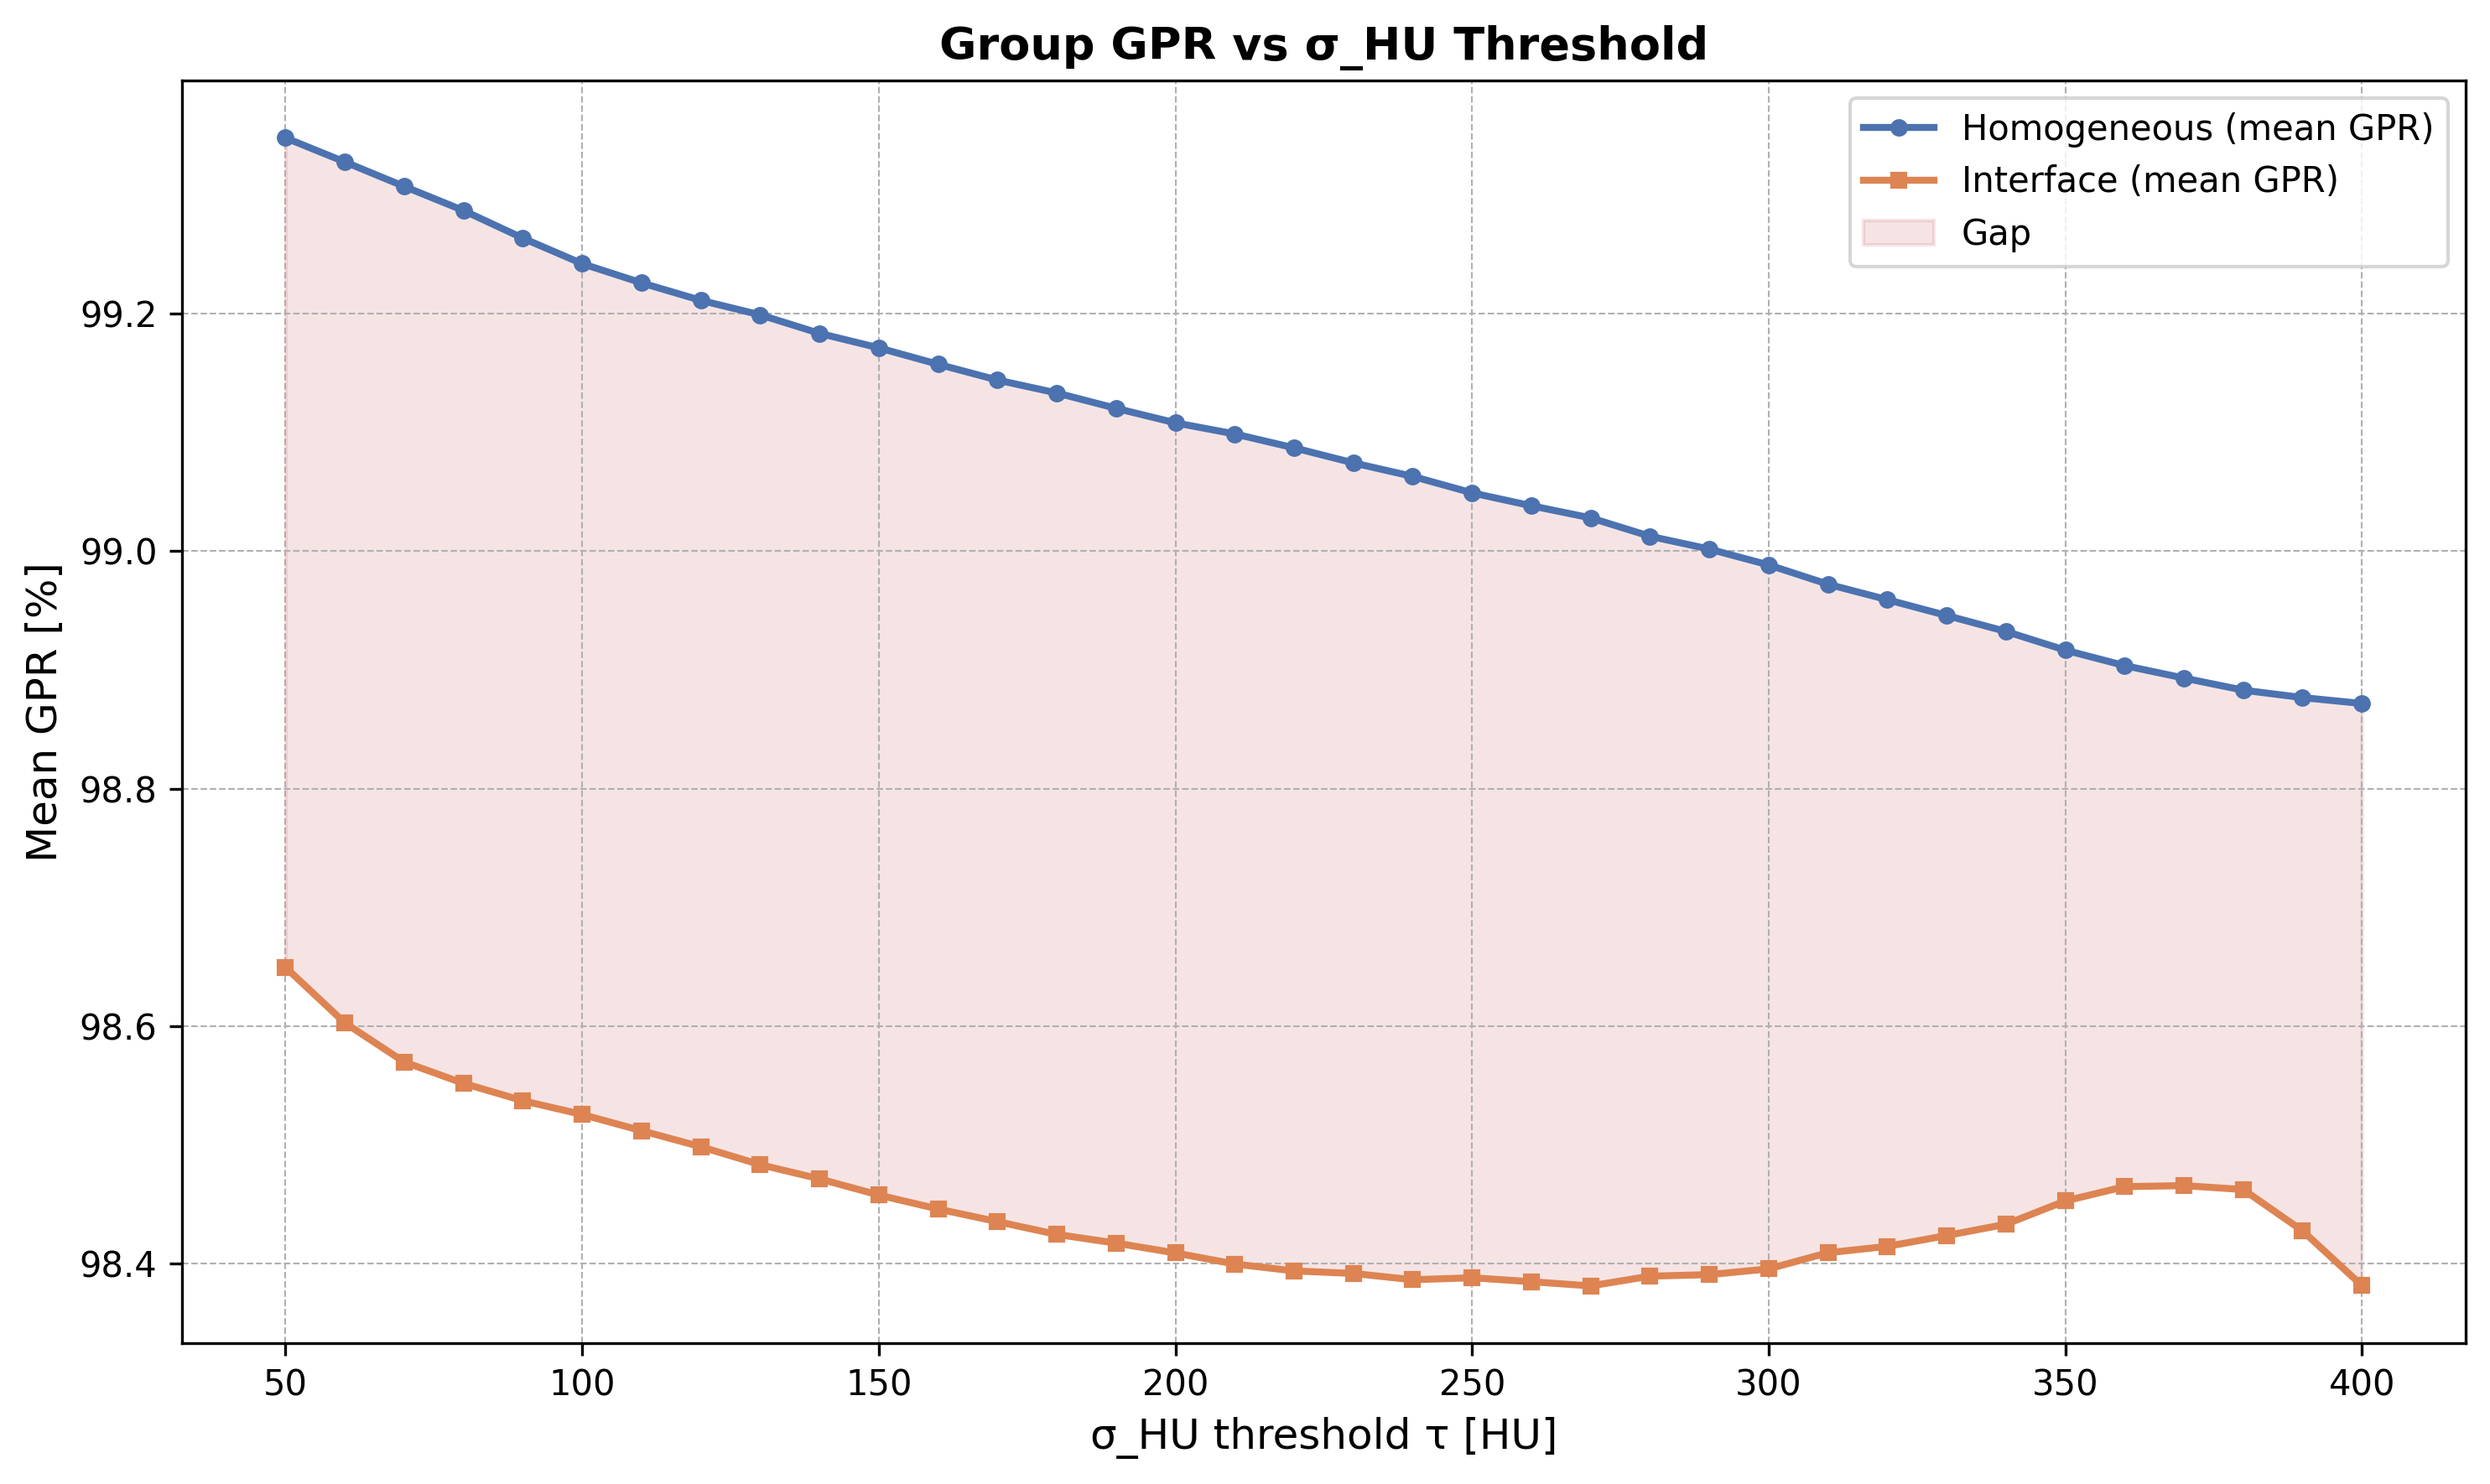
\includegraphics[width=0.68\textwidth]{sweep/group_gpr_vs_tau.png}
  \end{center}
  \vspace{-4pt}
  {\small Both curves decline slightly as $\tau$ increases (homogeneous
   group absorbs borderline cases), but the interface curve always sits
   \emph{below} the homogeneous curve.  The shaded gap is persistent.}
\end{frame}

% ── Result: all metrics ─────────────────────────────────────
\begin{frame}[shrink=10]{All-Metric Gaps vs.\ $\tau$ ($r = \SI{10}{mm}$)}
  \begin{center}
    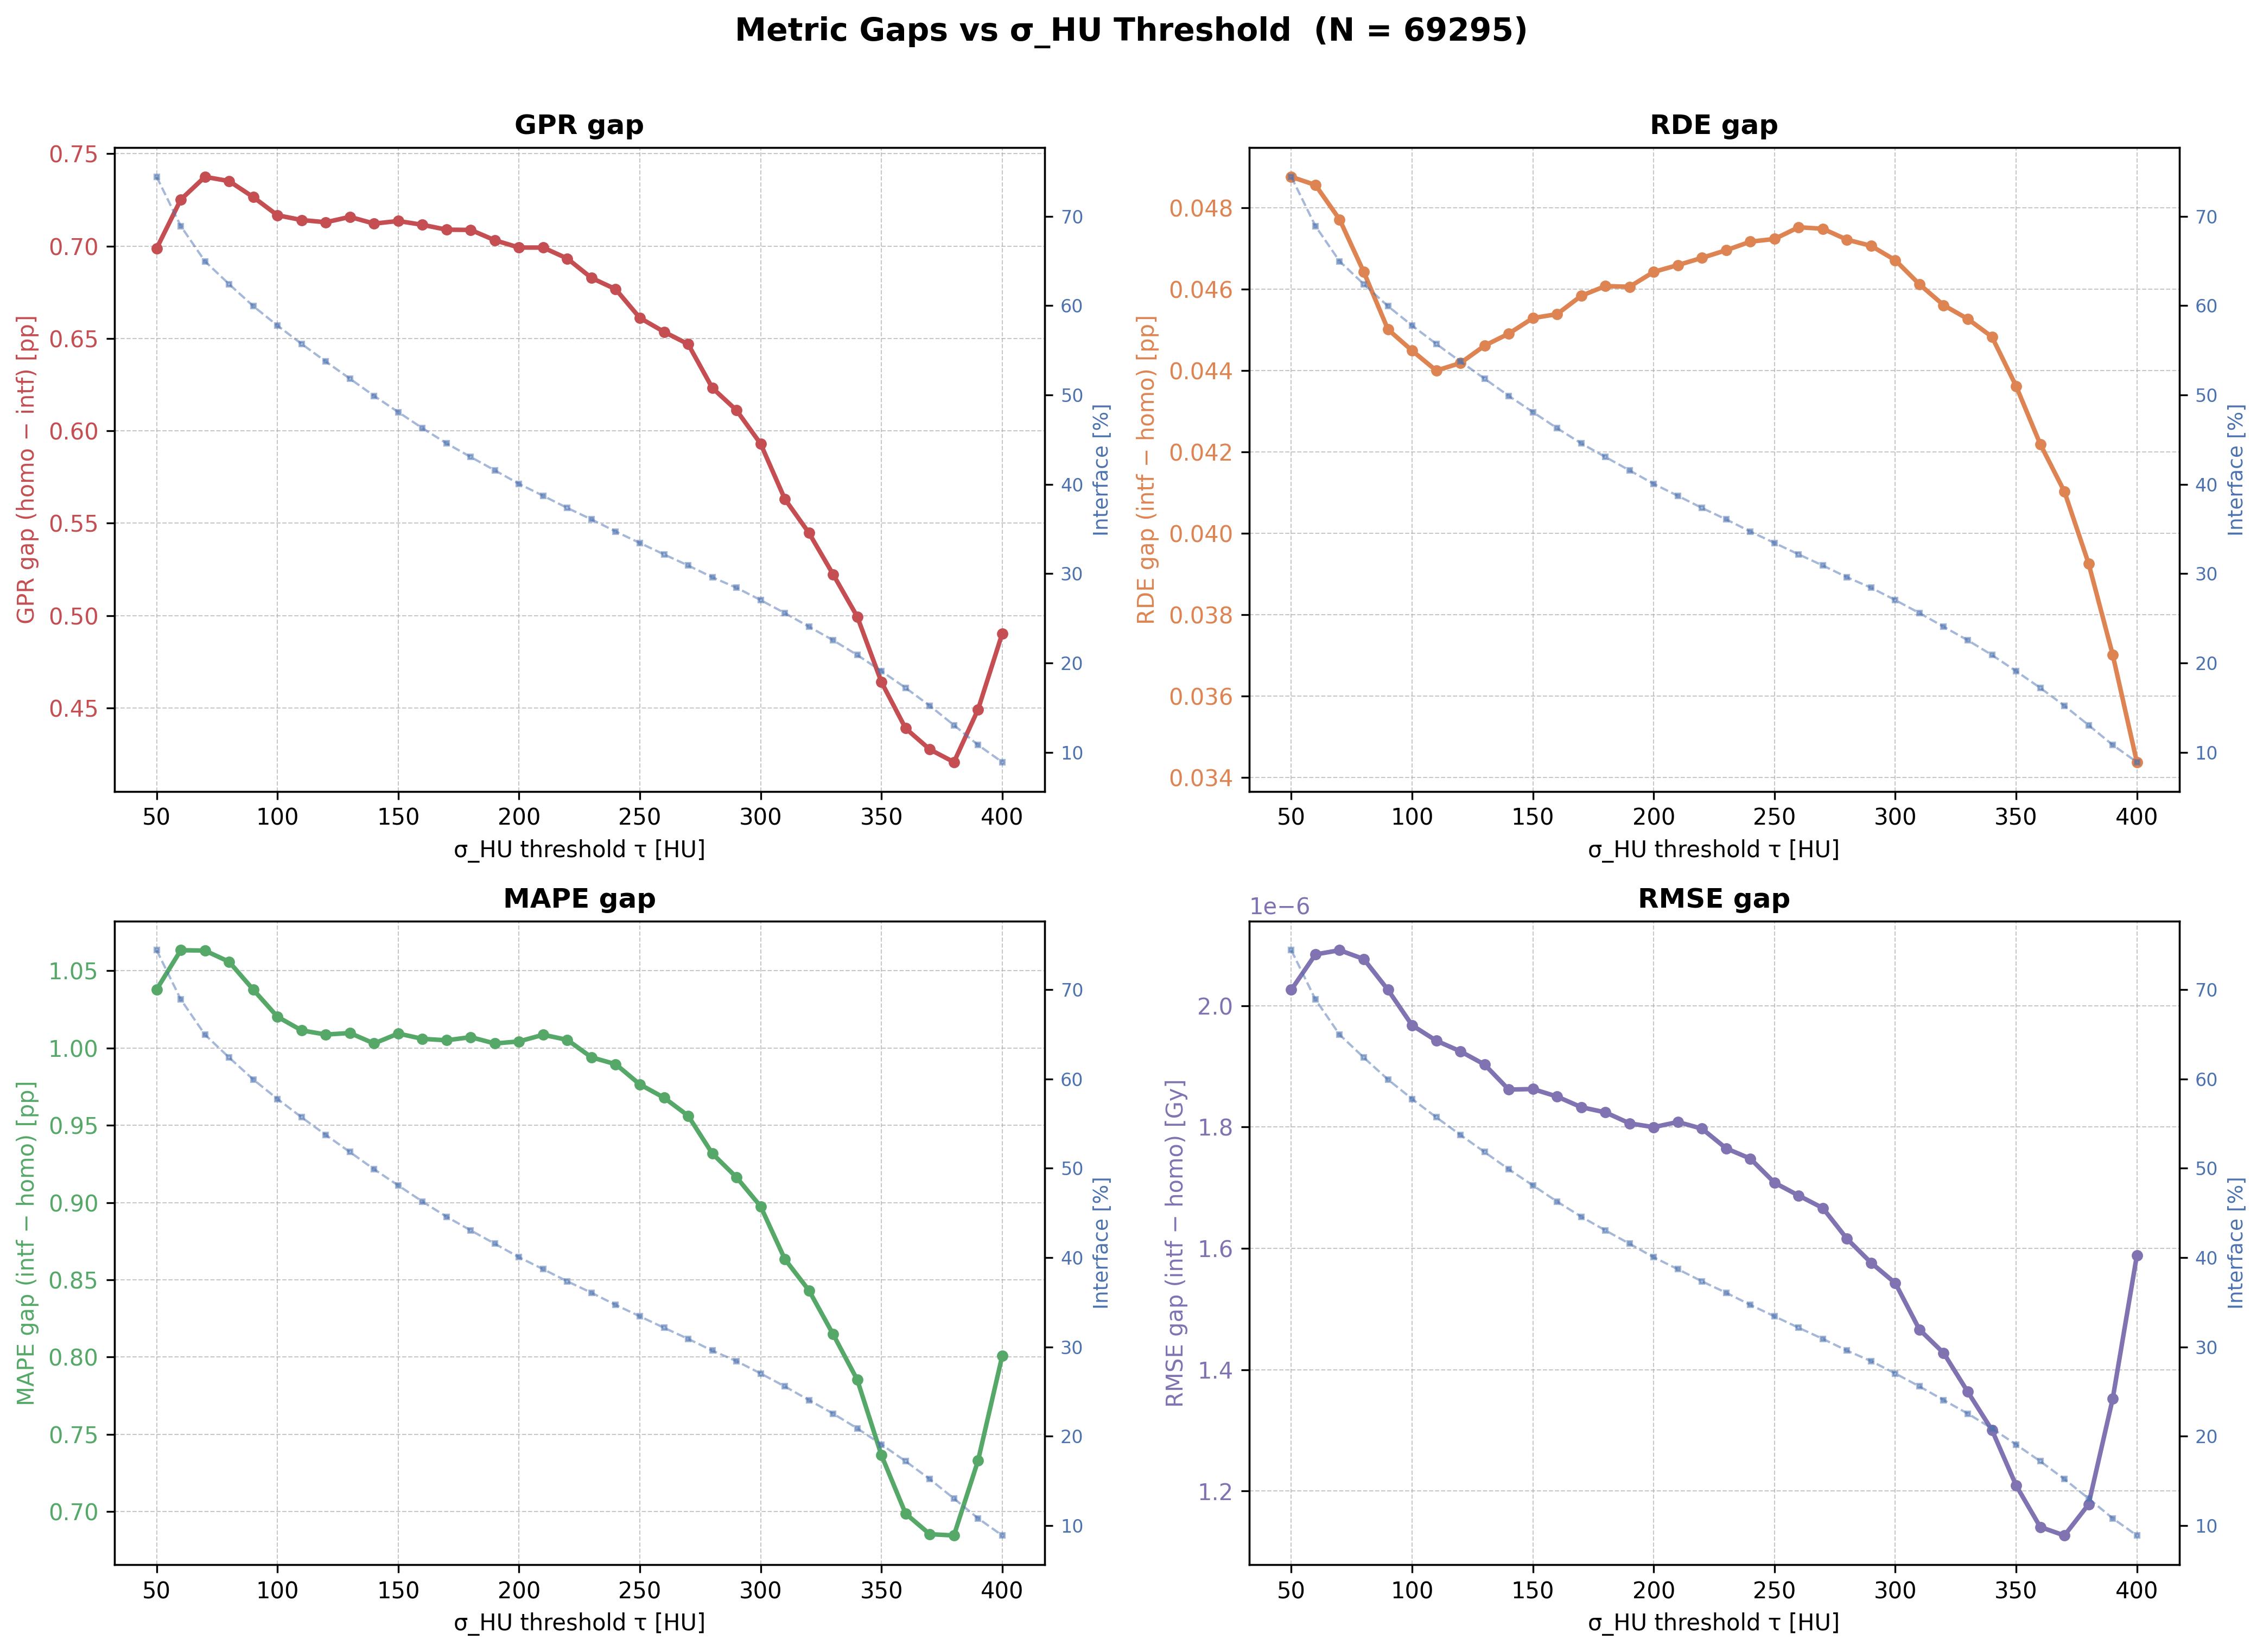
\includegraphics[width=0.62\textwidth]{sweep/all_metric_gaps_vs_tau.png}
  \end{center}
  \vspace{-4pt}
  {\small All four metrics confirm the same pattern: the interface group
   performs worse at \emph{every} threshold.  The RDE and MAPE gaps are
   remarkably flat, while the GPR and RMSE gaps show a gentle decline
   at extreme thresholds where the interface class becomes very small.}
\end{frame}

% ── Sweep discussion ────────────────────────────────────────
\begin{frame}[shrink=5]{Threshold Sweep — Key Findings}
  \begin{columns}[T]
    \begin{column}{0.48\textwidth}
      \textbf{Quantitative highlights:}
      \begin{table}
        \centering\small
        \begin{tabular}{lcc}
          \toprule
          $\tau$ [HU] & $\Delta_{\text{GPR}}$ [pp] & Intf.\ [\%] \\
          \midrule
           70 & 0.74 & 65.0 \\
          100 & 0.72 & 57.8 \\
          150 & 0.71 & 48.1 \\
          200 & 0.70 & 40.0 \\
          250 & 0.66 & 33.4 \\
          300 & 0.59 & 27.0 \\
          380 & 0.42 & 13.0 \\
          \bottomrule
        \end{tabular}
      \end{table}
    \end{column}
    \begin{column}{0.48\textwidth}
      \textbf{Interpretation:}
      \begin{itemize}\setlength{\itemsep}{3pt}
        \item The GPR gap is \textbf{not an artefact} of the threshold
              choice — it persists from $\tau = 50$ to \SI{400}{HU}.
        \item At low $\tau$, a large fraction is labelled
              interface, diluting the group with near-threshold cases,
              yet the gap remains $>$\SI{0.7}{pp}.
        \item At high $\tau$, only the most heterogeneous beamlets
              survive, but the interface group is too small for the gap
              to grow further.
        \item The \textbf{sweet spot} around $\tau \approx 70$–\SI{150}{HU}
              maximises the gap while keeping a large, statistically
              meaningful interface class.
      \end{itemize}
    \end{column}
  \end{columns}
\end{frame}

% ════════════════════════════════════════════════════════════
\section{Discussion}
% ════════════════════════════════════════════════════════════

\begin{frame}[shrink=5]{Discussion}
  \textbf{Summary of findings:}
  \begin{enumerate}\setlength{\itemsep}{2pt}
    \item A substantial fraction of the training set (\textbf{24--40\%},
          depending on $r$) consists of interface beamlets.
    \item Across \emph{all} four quality metrics, interface beamlets
          produce \textbf{systematically worse} predictions.
    \item The performance gap is \textbf{robust} to the choice of
          neighbourhood radius — it persists at both $r = 5$ and
          \SI{10}{mm}.
    \item Multiple heterogeneity features ($\sigma_{\text{HU}}$, TV)
          correlate with prediction error, suggesting the effect is
          physical rather than an artefact of the metric definition.
    \item The threshold sweep confirms that the gap is
          \textbf{not sensitive to $\tau$}: it remains positive over the
          entire $[50, 400]$\,HU range, peaking at $\approx$\SI{0.74}{pp}
          (GPR) near $\tau = \SI{70}{HU}$.
  \end{enumerate}

  \vspace{4pt}
  \textbf{Implications for model improvement:}
  \begin{itemize}\setlength{\itemsep}{2pt}
    \item \textbf{Data augmentation} — oversample interface cases during
          training to reduce the performance gap.
    \item \textbf{Architecture} — investigate attention mechanisms that
          can better handle density discontinuities.
    \item \textbf{Uncertainty quantification} — flag interface beamlets
          for downstream QA review.
    \item \textbf{Stratified evaluation} — always report metrics
          separately for interface vs.\ homogeneous subsets.
  \end{itemize}
\end{frame}

% ════════════════════════════════════════════════════════════
\section{Next Steps}
% ════════════════════════════════════════════════════════════

\begin{frame}{Next Steps}
  \begin{enumerate}
    \item \textbf{Additional anatomical sites} — repeat the analysis on
          the lung dataset, where tissue interfaces (lung--mediastinum)
          are even more prominent.
    \item \textbf{Multi-feature classification} — replace the binary
          $\sigma_{\text{HU}}$ threshold with a multi-feature classifier
          (e.g.\ $\sigma_{\text{HU}}$ + TV + CV) and examine ROC for
          predicting ``hard'' beamlets (GPR $<$ \SI{95}{\percent}).
    \item \textbf{Exclude worst offenders} — systematically remove the
          worst-predicted interface beamlets from training and measure
          whether retraining improves global metrics.
    \item \textbf{Energy-stratified analysis} — investigate whether the
          interface effect is stronger at specific energies (shallow
          vs.\ deep Bragg peaks).
    \item \textbf{Threshold sweep on $r = \SI{5}{mm}$ data} — verify
          that the gap-vs-$\tau$ curve retains the same shape with the
          smaller neighbourhood.
  \end{enumerate}
\end{frame}

% ── Closing ─────────────────────────────────────────────────
\begin{frame}[plain]
  \begin{center}
    \vspace{2cm}
    {\Huge\color{tudelft} Thank you}\\[12pt]
    {\large Questions \& discussion}\\[20pt]
    {\small Mikołaj Stryja \textbar{} \texttt{m.j.stryja@tudelft.nl}}
  \end{center}
\end{frame}

\end{document}